\chapter{Integration in das vorhandene System}
\label{ch:Implementierung}
	Um die in Kapitel \ref{sec: Reglung und autonomes Fahren} beschriebenen Probleme in dem Anlaufverhalten des ALF
	entgegenzuwirken, wird zur bereits bestehenden Drehmomentregelung eine übergeordnete Drehzahl- und Lageregelung implementiert. Grundlage für den Reglerentwurf bilden die Übertragungsfunktionen der Antriebe. Diese werden mit den in Kapitel \ref{sec: Regelung} beschriebenen Testfunktionen und anschließender Annäherung ermittelt. Die ungewollten Rotationen werden durch die übergeordneten Regelkreise ausgeregelt, dadurch hat das ALF ein stabiles Fahrverhalten. Dieses ist notwendig um definierterte Bewegungsbefehle mit der in dem Lastenheft geforderten Präzision abzufahren.

	\section{Analyse und Regelung des Fahrverhaltens}
	\label{sec:Schlupfregelung}

	Um das Systemverhalten der vorhandenen Antriebe zu analysieren wird eine Sprungantwort aufgenommen,
	indem der maximale Drehmomentsollwert an die Motorcontroller
	gesendet und die resultierenden Drehzahlen der Motoren aufgezeichnet wurde. Die Sprungantworten wurden gleichzeitig unter Last im Labor des Instituts für Systemtechnik aufgenommen. Die Last besteht lediglich aus dem Eigengewicht des Fahrzeugs. Die Abbildungen \ref{fig: brr}, \ref{fig: blr}, \ref{fig: frr} und \ref{fig: flr} zeigen die aufgenommenen Sprungantworten der einzelnen Antriebe
			
				\begin{figure}[H]
				\centering
				\begin{tikzpicture}[
				]
				\begin{axis}[
				width=12cm,
				height=7cm,
				grid = both,
				grid style={line width=.1pt, draw=gray!10},
				axis y line*=right,
				ylabel near ticks, %ylabel pos
				yticklabel pos=right,
				xmin=4.5, xmax=7.5, 
				ymin=-250, ymax=5500,
				ticklabel style={% gilt für x und y
					/pgf/number format/.cd,
					use comma,% Komma als Dezimaltrenner
					1000 sep = {}% keine Tausendertrennung 
				},
				ylabel={Drehzahl \textit{n} in min$^{\mathrm{-1}}$},
				axis x line*=bottom,
				%every axis plot/.append style={line width=1.0pt}
				]
				\addplot[smooth,black, line width=0.8pt]  table [col sep=comma] from {brr.csv};
				\label{plotbrr}
				\end{axis}
				\begin{axis}[
				width=12cm,
				height=7cm,
				axis y line*=left,
				 ticklabel style={% gilt für x und y
					/pgf/number format/.cd,
					use comma,% Komma als Dezimaltrenner
					1000 sep = {}% keine Tausendertrennung 
				},
				xlabel={$\text{Zeit } \textit{t} \text{ in Sekunden}$},
				ylabel={Drehmoment $M_{soll}$ in \%M$_{\mathrm{max}}$},
				axis x line*=bottom,
				xmin=4.5, xmax=7.5, 
				ymin=-5, ymax=110,
				%every axis plot/.append style={line width=1.0pt}
				legend pos=south east,
				]
				
				\addlegendentry{Soll-Drehmoment}; % legende1
				\addplot[gray, line width=0.8pt]  table [col sep=comma] from {brs.csv};
				\addlegendimage{/pgfplots/refstyle=plotbrr};				
				\addlegendentry{Ist-Drehzahl} ;%legende 2;
				%\addlegendentry{plot 1}
				\end{axis}
				\end{tikzpicture}
				\caption{Sprungantwort des Motors vorne rechts und maximale  sprungförmige Drehmomentvorgabe. Bei der Sollwertvorgabe handelt es sich um einen prozentualen Anteil des maximal möglichen Drehmoment. Die Stufe an dem sprungförmigen Eingangssignal entsteht durch die Eingabe des Sollwerts über den Joystick. Mit diesem Eingabegerät ist es nicht möglich einen idealen Einheitssprung zu erzeugen, wie die Sprungfunktion $u(t)$ aus Kapitel \ref{sec: Regelung} vorsieht. Für weitere Analysen wird dieser Fehler vernachlässigt.}
				\label{fig: brr}
			\end{figure}
		
		
		
				\begin{figure}[H]
				\centering
								\begin{tikzpicture}[
				]
				\begin{axis}[
				width=12cm,
				height=7cm,
				grid = both,
				grid style={line width=.1pt, draw=gray!10},
				axis y line*=right,
				ylabel near ticks, %ylabel pos
				yticklabel pos=right,
				xmin=4.5, xmax=7.5, 
				ymin=-250, ymax=5500,
				ticklabel style={% gilt für x und y
					/pgf/number format/.cd,
					use comma,% Komma als Dezimaltrenner
					1000 sep = {}% keine Tausendertrennung 
				},
				ylabel={Drehzahl \textit{n} in min$^{\mathrm{-1}}$},
				axis x line*=bottom,
				%every axis plot/.append style={line width=1.0pt}
				]
				\addplot[smooth,black, line width=0.8pt]  table [col sep=comma] from {blr.csv};
				\label{plotblr}
				\end{axis}
				\begin{axis}[
				width=12cm,
				height=7cm,
				axis y line*=left,
				ticklabel style={% gilt für x und y
					/pgf/number format/.cd,
					use comma,% Komma als Dezimaltrenner
					1000 sep = {}% keine Tausendertrennung 
				},
				xlabel={$\text{Zeit } \textit{t} \text{ in Sekunden}$},
				ylabel={Drehmoment $M_{soll}$ in \%M$_{\mathrm{max}}$},
				axis x line*=bottom,
				xmin=4.5, xmax=7.5, 
				ymin=-5, ymax=110,
				%every axis plot/.append style={line width=1.0pt}
				legend pos=south east,
				]
				
				\addlegendentry{Soll-Drehmoment}; % legende1
				\addplot[gray, line width=0.8pt]  table [col sep=comma] from {bls.csv};
				\addlegendimage{/pgfplots/refstyle=plotblr};				
				\addlegendentry{Ist-Drehzahl} ;%legende 2;
				%\addlegendentry{plot 1}
				\end{axis}
				\end{tikzpicture}
				\caption{Sprungantwort des Motors hinten links und maximale sprungförmige Drehmomentvorgabe.}
				\label{fig: blr}
			\end{figure}
			
			\begin{figure}[H]
				\centering
								\begin{tikzpicture}[
				]
				\begin{axis}[
				width=12cm,
				height=7cm,
				grid = both,
				grid style={line width=.1pt, draw=gray!10},
				axis y line*=right,
				ylabel near ticks, %ylabel pos
				yticklabel pos=right,
				xmin=4.5, xmax=7.5, 
				ymin=-250, ymax=5500,
				ticklabel style={% gilt für x und y
					/pgf/number format/.cd,
					use comma,% Komma als Dezimaltrenner
					1000 sep = {}% keine Tausendertrennung 
				},
				ylabel={Drehzahl \textit{n} in min$^{\mathrm{-1}}$},
				axis x line*=bottom,
				%every axis plot/.append style={line width=1.0pt}
				]
				\addplot[smooth,black, line width=0.8pt]  table [col sep=comma] from {frr.csv};
				\label{plotfrr}
				\end{axis}
				\begin{axis}[
				width=12cm,
				height=7cm,
				axis y line*=left,
				ticklabel style={% gilt für x und y
					/pgf/number format/.cd,
					use comma,% Komma als Dezimaltrenner
					1000 sep = {}% keine Tausendertrennung 
				},
				xlabel={$\text{Zeit } \textit{t} \text{ in Sekunden}$},
				ylabel={Drehmoment $M_{soll}$ in \%M$_{\mathrm{max}}$},
				axis x line*=bottom,
				xmin=4.5, xmax=7.5, 
				ymin=-5, ymax=110,
				%every axis plot/.append style={line width=1.0pt}
				legend pos=south east,
				]
				
				\addlegendentry{Soll-Drehmoment}; % legende1
				\addplot[gray, line width=0.8pt]  table [col sep=comma] from {frs.csv};
				\addlegendimage{/pgfplots/refstyle=plotfrr};				
				\addlegendentry{Ist-Drehzahl} ;%legende 2;
				%\addlegendentry{plot 1}
				\end{axis}
				\end{tikzpicture}
				\caption{Sprungantwort des Motors vorne rechts und maximale sprungförmige Drehmomentvorgabe.}
				\label{fig: frr}
			\end{figure}
	
				\begin{figure}[H]
		\centering
					\begin{tikzpicture}[
	]
	\begin{axis}[
	width=12cm,
	height=7cm,
	grid = both,
	grid style={line width=.1pt, draw=gray!10},
	axis y line*=right,
	ylabel near ticks, %ylabel pos
	yticklabel pos=right,
	xmin=4.5, xmax=7.5, 
	ymin=-250, ymax=5500,
	ticklabel style={% gilt für x und y
		/pgf/number format/.cd,
		use comma,% Komma als Dezimaltrenner
		1000 sep = {}% keine Tausendertrennung 
	},
	ylabel={Drehzahl \textit{n} in min$^{\mathrm{-1}}$},
	axis x line*=bottom,
	%every axis plot/.append style={line width=1.0pt}
	]
	\addplot[smooth,black, line width=0.8pt]  table [col sep=comma] from {flr.csv};
	\label{plotflr}
	\end{axis}
	\begin{axis}[
	width=12cm,
	height=7cm,
	axis y line*=left,
	ticklabel style={% gilt für x und y
		/pgf/number format/.cd,
		use comma,% Komma als Dezimaltrenner
		1000 sep = {}% keine Tausendertrennung 
	},
	xlabel={$\text{Zeit } \textit{t} \text{ in Sekunden}$},
	ylabel={Drehmoment $M_{soll}$ in \%M$_{\mathrm{max}}$},
	axis x line*=bottom,
	xmin=4.5, xmax=7.5, 
	ymin=-5, ymax=110,
	%every axis plot/.append style={line width=1.0pt}
	legend pos=south east,
	]
	
	\addlegendentry{Soll-Drehmoment}; % legende1
	\addplot[gray, line width=0.8pt]  table [col sep=comma] from {fls.csv};
	\addlegendimage{/pgfplots/refstyle=plotflr};				
	\addlegendentry{Ist-Drehzahl} ;%legende 2;
	%\addlegendentry{plot 1}
	\end{axis}
	\end{tikzpicture}
		\caption{Sprungantwort des Motors vorne links und maximale sprungförmige Drehmomentvorgabe. }
		\label{fig: flr}
	\end{figure}
			
			
			Anhand der Sprungantworten aus den Abbildungen \ref{fig: brr}, \ref{fig: blr}, \ref{fig: frr} und \ref{fig: flr} und der Vernachlässigung von Totzeiten, lässt sich das Verhalten von Verzögerungsgliedern 2. Ordnung identifizieren. Deren Übertragungsfunktion mit der allgemeinen Form 
			
			\begin{equation}
					G(s)=\frac{k_s}{T^2s^2+2DTs+1}
					\label{eq:pt2}
			\end{equation}\newline
			
			beschrieben wird \cite{unbehauen,lunze}. Eine Berechnung der Fehlerleistung des angenäherten Signals im Verhältnis zu der gemessenen Ist-Drehzahl ergab für die vier Antriebe einen Wert von $0{,}7$\%. Daher ist für die Realisierung der im Lastenheft beschriebenen Anforderungen an die Drehzahlregelung eine Optimierung der Annäherung nicht notwendig.
			Durch diese Identifikation werden mithilfe der Matlab Funktion \textit{Transfer Function Estimation} (tfest) die Übertragungsfunktionen für die Sprungantworten aus den Abbildungen \ref{fig: brr}, \ref{fig: blr}, \ref{fig: frr} und \ref{fig: flr} geschätzt \cite{tfest}. Für die Anwendung von \textit{tfest} sind Kenntnisse über die Anzahl der Pol- und Nullstellen der Übertragungsfunktion erforderlich. Bei einem Verzögerungsglied 2. Ordnung treten aufgrund der gebrochen-rationalen Funktion aus Gleichung (\ref{eq:pt2}) zwei Polstellen und keine Nullstelle auf \cite{unbehauen}. Durch Anwenden der Funktion \textit{tfest} erhält man die Übertragungsfunktionen \ref{eq: g1est}, \ref{eq: g2est}, \ref{eq: g3est} und \ref{eq: g4est}: 
			
			\begin{align}
			\label{eq: g1est}
			G_{1}(s)=\frac{248{,}7}{s^2+3{,}074s+5{,}101}\\\nonumber\\
			\label{eq: g2est}
			G_{2}(s)=\frac{232{,}4}{s^2+3{,}005s+4{,}702}\\\nonumber\\
			\label{eq: g3est}
			G_{3}(s)=\frac{314}{s^2+3{,}816s+6{,}208}\\\nonumber\\
			\label{eq: g4est}
			G_{4}(s)=\frac{251{,}6}{s^2+3{,}175s+5{,}96}
			\end{align}\newline
			Eine Simulation zur Verifikation der approximierten Übertragungsfunktionen in \textit{Simulink}, mit den gleichen Simulationsparametern wie bei der Aufnahme der Sprungantwort, liefert ein äquivalentes Übertragungsverhalten der geschätzten und experimentell ermittelten Sprungantworten und ist in den Abbildungen \ref{fig: gbrest}, \ref{fig: gblest}, \ref{fig: gfrest} und \ref{fig: gflest} zu sehen.
			 
		\begin{figure}[H]
			\centering
				\begin{tikzpicture}[
]
\begin{axis}[
width=12cm,
height=7cm,
grid = both,
grid style={line width=.1pt, draw=gray!10},
axis y line*=right,
ylabel near ticks, %ylabel pos
yticklabel pos=right,
xmin=4.5, xmax=7.5, 
ymin=-250, ymax=5500,
ticklabel style={% gilt für x und y
	/pgf/number format/.cd,
	use comma,% Komma als Dezimaltrenner
	1000 sep = {}% keine Tausendertrennung 
},
ylabel={Drehzahl \textit{n} in min$^{\mathrm{-1}}$},
axis x line*=bottom,
%every axis plot/.append style={line width=1.0pt}
]
\addplot[smooth,black, line width=0.8pt]  table [col sep=comma] from {brr.csv};
\label{plotgbrr2}
\addplot[smooth,red, line width=0.8pt]  table [col sep=comma] from {gbrest.csv};
\label{plotgbrest}
\end{axis}
\begin{axis}[
width=12cm,
height=7cm,
axis y line*=left,
ticklabel style={% gilt für x und y
	/pgf/number format/.cd,
	use comma,% Komma als Dezimaltrenner
	1000 sep = {}% keine Tausendertrennung 
},
xlabel={$\text{Zeit } \textit{t} \text{ in Sekunden}$},
ylabel={Drehmoment $M_{soll}$ in \%M$_{\mathrm{max}}$},
axis x line*=bottom,
xmin=4.5, xmax=7.5, 
ymin=-5, ymax=110,
%every axis plot/.append style={line width=1.0pt}
legend pos=south east,
]

\addlegendentry{Soll-Drehmoment}; % legende1
\addplot[gray, line width=0.8pt]  table [col sep=comma] from {brs.csv};
\addlegendimage{/pgfplots/refstyle=plotbrr2};				
\addlegendentry{Ist-Drehzahl} ;%legende 2;
\addlegendimage{/pgfplots/refstyle=plotgbrest};	
\addlegendentry{Ist-Drehzahl angenähert} ;%legende 2;
%\addlegendentry{plot 1}
\end{axis}
\end{tikzpicture}
	\caption{Sprungantwort des Motors hinten rechts mit der geschäzten Übertragungsfunktion $G_{1}(s)$ und dem Eingangssignal aus der experimentell ermittelten Sprungantwort. Der zeitliche Verlauf der Übertragungsfunktion wurde mit Hilfe von \textit{Simulink} ermittelt. Dafür wurde die Simulationszeit, Schrittweite und der Start des Eingangssignals der originalen Sprungantwort als Simulationsparameter in eingegeben.}
	\label{fig: gbrest}
\end{figure}
	
	
	\begin{figure}[H]
		\centering
					\begin{tikzpicture}[
	]
	\begin{axis}[
	width=12cm,
	height=7cm,
	grid = both,
	grid style={line width=.1pt, draw=gray!10},
	axis y line*=right,
	ylabel near ticks, %ylabel pos
	yticklabel pos=right,
	xmin=4.5, xmax=7.5, 
	ymin=-250, ymax=5500,
	ticklabel style={% gilt für x und y
		/pgf/number format/.cd,
		use comma,% Komma als Dezimaltrenner
		1000 sep = {}% keine Tausendertrennung 
	},
	ylabel={Drehzahl \textit{n} in min$^{\mathrm{-1}}$},
	axis x line*=bottom,
	%every axis plot/.append style={line width=1.0pt}
	]
	\addplot[smooth,black, line width=0.8pt]  table [col sep=comma] from {blr.csv};
	\label{plotgblr2}
	\addplot[smooth,red, line width=0.8pt]  table [col sep=comma] from {gblest.csv};
	\label{plotgblest}
	\end{axis}
	\begin{axis}[
	width=12cm,
	height=7cm,
	axis y line*=left,
	ticklabel style={% gilt für x und y
		/pgf/number format/.cd,
		use comma,% Komma als Dezimaltrenner
		1000 sep = {}% keine Tausendertrennung 
	},
	xlabel={$\text{Zeit } \textit{t} \text{ in Sekunden}$},
	ylabel={Drehmoment $M_{soll}$ in \%M$_{\mathrm{max}}$},
	axis x line*=bottom,
	xmin=4.5, xmax=7.5, 
	ymin=-5, ymax=110,
	%every axis plot/.append style={line width=1.0pt}
	legend pos=south east,
	]
	
	\addlegendentry{Soll-Drehmoment}; % legende1
	\addplot[gray, line width=0.8pt]  table [col sep=comma] from {bls.csv};
	\addlegendimage{/pgfplots/refstyle=plotblr2};				
	\addlegendentry{Ist-Drehzahl} ;%legende 2;
	\addlegendimage{/pgfplots/refstyle=plotgblest};	
	\addlegendentry{Ist-Drehzahl angenähert} ;%legende 2;
	%\addlegendentry{plot 1}
	\end{axis}
	\end{tikzpicture}
		\caption{Sprungantwort des Motors hinten links mit der geschätzten Übertragungsfunktion $G_{2}(s)$ und dem Eingangssignal aus der experimentell ermittelten Sprungantwort.}
		\label{fig: gblest}
	\end{figure}
	
		\begin{figure}[H]
		\centering
					\begin{tikzpicture}[
	]
	\begin{axis}[
	width=12cm,
	height=7cm,
	grid = both,
	grid style={line width=.1pt, draw=gray!10},
	axis y line*=right,
	ylabel near ticks, %ylabel pos
	yticklabel pos=right,
	xmin=4.5, xmax=7.5, 
	ymin=-250, ymax=5500,
	ticklabel style={% gilt für x und y
		/pgf/number format/.cd,
		use comma,% Komma als Dezimaltrenner
		1000 sep = {}% keine Tausendertrennung 
	},
	ylabel={Drehzahl \textit{n} in min$^{\mathrm{-1}}$},
	axis x line*=bottom,
	%every axis plot/.append style={line width=1.0pt}
	]
	\addplot[smooth,black, line width=0.8pt]  table [col sep=comma] from {frr.csv};
	\label{plotgfrr2}
	\addplot[smooth,red, line width=0.8pt]  table [col sep=comma] from {gfrest.csv};
	\label{plotgfrest}
	\end{axis}
	\begin{axis}[
	width=12cm,
	height=7cm,
	axis y line*=left,
	ticklabel style={% gilt für x und y
		/pgf/number format/.cd,
		use comma,% Komma als Dezimaltrenner
		1000 sep = {}% keine Tausendertrennung 
	},
	xlabel={$\text{Zeit } \textit{t} \text{ in Sekunden}$},
	ylabel={Drehmoment $M_{soll}$ in \%M$_{\mathrm{max}}$},
	axis x line*=bottom,
	xmin=4.5, xmax=7.5, 
	ymin=-5, ymax=110,
	%every axis plot/.append style={line width=1.0pt}
	legend pos=south east,
	]
	
	\addlegendentry{Soll-Drehmoment}; % legende1
	\addplot[gray, line width=0.8pt]  table [col sep=comma] from {frs.csv};
	\addlegendimage{/pgfplots/refstyle=plotfrr2};				
	\addlegendentry{Ist-Drehzahl} ;%legende 2;
	\addlegendimage{/pgfplots/refstyle=plotgfrest};	
	\addlegendentry{Ist-Drehzahl angenähert} ;%legende 2;
	%\addlegendentry{plot 1}
	\end{axis}
	\end{tikzpicture}
		\caption{Sprungantwort des Motors vorne rechts mit der geschätzten Übertragungsfunktion $G_{3}(s)$ und dem Eingangssignal aus der experimentell ermittelten Sprungantwort.}
		\label{fig: gfrest}
	\end{figure}
		 
		\begin{figure}[H]
		 	\centering
					\begin{tikzpicture}[
	]
	\begin{axis}[
	width=12cm,
	height=7cm,
	grid = both,
	grid style={line width=.1pt, draw=gray!10},
	axis y line*=right,
	ylabel near ticks, %ylabel pos
	yticklabel pos=right,
	xmin=4.5, xmax=7.5, 
	ymin=-250, ymax=5500,
	ticklabel style={% gilt für x und y
		/pgf/number format/.cd,
		use comma,% Komma als Dezimaltrenner
		1000 sep = {}% keine Tausendertrennung 
	},
	ylabel={Drehzahl \textit{n} in min$^{\mathrm{-1}}$},
	axis x line*=bottom,
	%every axis plot/.append style={line width=1.0pt}
	]
	\addplot[smooth,black, line width=0.8pt]  table [col sep=comma] from {flr.csv};
	\label{plotgflr2}
	\addplot[smooth,red, line width=0.8pt]  table [col sep=comma] from {gflest.csv};
	\label{plotgflest}
	\end{axis}
	\begin{axis}[
	width=12cm,
	height=7cm,
	axis y line*=left,
	ticklabel style={% gilt für x und y
		/pgf/number format/.cd,
		use comma,% Komma als Dezimaltrenner
		1000 sep = {}% keine Tausendertrennung 
	},
	xlabel={$\text{Zeit } \textit{t} \text{ in Sekunden}$},
	ylabel={Drehmoment $M_{soll}$ in \%M$_{\mathrm{max}}$},
	axis x line*=bottom,
	xmin=4.5, xmax=7.5, 
	ymin=-5, ymax=110,
	%every axis plot/.append style={line width=1.0pt}
	legend pos=south east,
	]
	
	\addlegendentry{Soll-Drehmoment}; % legende1
	\addplot[gray, line width=0.8pt]  table [col sep=comma] from {fls.csv};
	\addlegendimage{/pgfplots/refstyle=plotflr2};				
	\addlegendentry{Ist-Drehzahl} ;%legende 2;
	\addlegendimage{/pgfplots/refstyle=plotgflest};	
	\addlegendentry{Ist-Drehzahl angenähert} ;%legende 2;
	%\addlegendentry{plot 1}
	\end{axis}
	\end{tikzpicture}
		 	\caption{Sprungantwort des Motors vorne links mit der geschätzten Übertragungsfunktion $G_{4}(s)$ und dem Eingangssignal aus der experimentell ermittelten Sprungantwort.}
		 	\label{fig: gflest}
		 \end{figure}
		 
		 	Nac
			Die Übertragungsfunktionen werden in die Form aus Gleichung (\ref{eq:pt2}) umgestellt, so dass die Zeitkonstante und Dämpfung bestimmt werden kann. 
			%Das Zerlegender Übertragungsfunktion in zwei Pt1 Glieder um einen Regler mit demBetragsoptimum auszulegen ist in diesem Fall nicht möglich, da die Funktionzwei konjuiert Komplexe Pole mit negtivem Realteil aufweist.
			 
			 
			\begin{align}
			 \label{eq: g1tfest}
			  G_{1}(s)&=\frac{48{,}7551}{0{,}1815s^2+0{,}6026s+1} \rightarrow D_{1}=0{,}7071 \text{ und } T_{1}=0{,}4261\text{ s}\\\nonumber\\
			 \label{eq: g2tfest}
			 G_{2}(s)&=\frac{49{,}4258}{0{,}2127s^2+0{,}6391s+1} \rightarrow D_{2}=0{,}6929 \text{ und } T_{2}=0{,}4612\text{ s}\\\nonumber\\
			 \label{eq: g3tfest}
			 G_{3}(s)&=\frac{50{,}5799}{0{,}1611s^2+0{,}6147s+1} \rightarrow D_{3}=0{,}7691 \text{ und } T_{3}=0{,}4014\text{ s}\\\nonumber\\
			 \label{eq: g4tfest}
			 G_{4}(s)&=\frac{48{,}4219}{0{,}1925s^2+0{,}6110s+1} \rightarrow D_{4}=0{,}6965 \text{ und } T_{4}=0{,}4387\text{ s}
			 \end{align}\newline
			 
			 
			
			 
			Die nun vorhandenen mathematische Modelle der Übertragungsfunktionen werden für die Simulation verschiedener Regler in \textit{Matlab/Simulink} und die anschließende Verwendung im ALF genutzt. Die Werte der Dämpfung D liegen zwischen null und eins, daraus resultiert ein schwingendes Verhalten der Übertragungsfunktion. Das abklingen des Schwingungsverlaufs wird durch diee Größe $T$ beschrieben und wird auch als Abklingzeitkonstante \cite{unbehauen}.
			
			
		\subsection{Regelung der Drehzahl}
		\label{sec: Drehzahlregelung}
		
		Die Drehzahlregelung wird mithilfe eines PI-Reglers realisiert, da dieser die Vorteile eines P- und I-Reglers vereint \cite{praktischeregelungstechnik}. Aufgrund des P-Anteils, reagiert der Regler unmittelbar und hat durch die zeitliche Integration der Regelabweichung keine bleibende Regeldifferenz. Durch die vorhandenen mathematische Modelle können verschiedene PI-Regler an den Regelstrecken simuliert werden. Es werden mehrere PI-Regler mit den Einstellregeln nach Chien, Hrones und Reswick aus Tabelle \ref{tab: reswick} und empirisch am Fahrverhalten ausgelegt und simuliert.
		
		
		\begin{table}[]
		\centering
		\begin{tabular}{|c|c|c|c|c|c|}
			\hline
			\multirow{2}{*}{Regler} & \multirow{2}{*}{} & \multicolumn{2}{c|}{Aperiodischer Regelverlauf}                   & \multicolumn{2}{c|}{Regelverlauf mit 20\% Überschwingen}                  \\ \cline{3-6} 
			&                   & Störung                         & Führung                         & Störungen                               & Führung                         \\ \hline
			P                       & $K_{p}$           & $0{,}3 \frac{T_{g}}{T_{u}K_{s}}$  & $0{,}3 \frac{T_{g}}{T_{u}K_{s}}$  & \textit{$0{,}7 \frac{T_{g}}{T_{u}K_{s}}$} & $0{,}7 \frac{T_{g}}{T_{u}K_{s}}$  \\ \hline
			\multirow{2}{*}{PI}     & $K_{p}$           & $0{,}6 \frac{T_{g}}{T_{u}K_{s}}$  & $0{,}35 \frac{T_{g}}{T_{u}K_{s}}$ & $0{,}7 \frac{T_{g}}{T_{u}K_{s}}$          & $0{,}6 \frac{T_{g}}{T_{u}K_{s}}$  \\ \cline{2-6} 
			& $T_{n}$           & $4T_{u}$                        & $1{,}2T_{g}$                      & $2T_{u}$                                & $4T_{u}$                        \\ \hline
			\multirow{3}{*}{PID}    & $K_{p}$           & $0{,}95 \frac{T_{g}}{T_{u}K_{s}}$ & $0{,}6 \frac{T_{g}}{T_{u}K_{s}}$  & \textit{$1{,}2 \frac{T_{g}}{T_{u}K_{s}}$} & $0{,}95 \frac{T_{g}}{T_{u}K_{s}}$ \\ \cline{2-6} 
			& $T_{n}$           & $2{,}4T_{u}$                      & $T_{g}$                         & \textit{$2T_{u}$}                       & $1{,}35T_{g}$                     \\ \cline{2-6} 
			& $T_{v}$           & $0{,}42T_{u}$                     & $0{,}5T_{u}$                      & $0{,}42T_{u}$                             & $0{,}47T_{u}$                     \\ \hline
		\end{tabular}
		\caption{Die Einstellregeln wurden von Chien, Hrones und Reswick für verschiedene Übertragungsfunktionen ermittelt. Die Einstellwerte sind für Führungs- und Störverhalten angegeben. Je nachdem, ob eine Störung möglichst schnell ausgeglichen werden, oder ob der Regler einem zeitlich veränderlichen Sollwert gut folgen soll. \cite{praktischeregelungstechnik}}
		\label{tab: reswick}
	\end{table}
		
 			Für die Einstellregeln sind Informationen über die Verzugszeit $T_{u}$ und die Anstiegszeit $T_{g}$ notwendig, diese Größen werden durch die Anwendung des  Wendetangentenverfahrens an der approximierten Regelstrecken gewonnen. Das Verfahren wird in dieser Bachelorarbeit für eine Übertragungsfunktion gezeigt, das vorgehen für die verbliebenen drei Regelstrecken ist analog. \cite{unbehauen,praktischeregelungstechnik}
		
				 		\begin{figure}[H]
			\centering
			\begin{tikzpicture}[
			]
			\begin{axis}[
				grid = both,
			grid style={line width=.1pt, draw=gray!10},
			width=12cm,
			height=7cm,
			axis y line*=right,
			ylabel near ticks, %ylabel pos
			yticklabel pos=right,
			xmin=4.5, xmax=7.5, 
			ymin=-250, ymax=5500,,
			ticklabel style={% gilt für x und y
				/pgf/number format/.cd,
				use comma,% Komma als Dezimaltrenner
				1000 sep = {}% keine Tausendertrennung 
			},
			ylabel={Drehzahl \textit{n} in min$^{\mathrm{-1}}$},
			axis x line*=bottom
			]
			%\addplot expression{4862};
		
			\addplot[red, line width=0.8pt]  table [col sep=comma] from {gbrest.csv};
			\label{brest}
				\addplot[black, line width=0.8pt]  table [col sep=comma] from {wende.csv};
			\label{wende}
			\addplot[black] [dash dot, line width=1.25pt]coordinates {(5.742,0) (5.742,5500) };
			\addplot[black] [dash dot, line width=1.25pt]coordinates {(4.795,0) (4.795,5500) };
			\addplot[black] [dash dot, line width=1.25pt]coordinates {(4.646,0) (4.646,5500) };
			\end{axis}
			\begin{axis}[
			width=12cm,
			height=7cm,
			axis y line*=left,
			ticklabel style={% gilt für x und y
				/pgf/number format/.cd,
				use comma,% Komma als Dezimaltrenner
				1000 sep = {}% keine Tausendertrennung 
			},
			xlabel={$\text{Zeit } \textit{t} \text{ in Sekunden}$},
			ylabel={Drehmoment $M_{soll}$ in \%M$_{\mathrm{max}}$},
			axis x line*=bottom,
			xmin=4.5, xmax=7.5, 
			ymin=-5, ymax=110,
			legend pos=south east
			]
			\addlegendimage{/pgfplots/refstyle=brest};
			\addlegendentry{Ist-Drehzahl angenähert} ;
			\addplot[gray, line width=0.8pt]  table [col sep=comma] from {brs.csv};
			\addlegendentry{Soll-Drehmoment}; 
			\addlegendimage{/pgfplots/refstyle=wende};
			\addlegendentry{Wendetangente} ;
			\end{axis}
 			\draw[<->,line width=0.8pt] (0.5,5.2) -- (1.0,5.2);
 			\draw[<->,line width=0.8pt] (0.5,5.2) -- (4.5,5.2);
 			\node[below] at (2.5,6){ $T_{g}$ };
 			\node[below] at (0.75,6){ $T_{u}$ };
			\end{tikzpicture}
			\caption{Angenährte Übertragungsfunktion des Antriebs hinten rechts mit Soll-Drehmoment und Wendetangente. Durch bestimmen und einzeichnen der Wendetangente wird die Verzugs- und Anstiegszeit ermittelt. In Punkt-Strich Form sind Hilfslinien eingezeichnet mit denen die Zeiten von der Zeitachse abgelesen werden können.}
			\label{fig: sprungantwort_wende}
		\end{figure}
		
		
			Mithilfe der in Abbildung \ref{fig: sprungantwort_wende} eingezeichneten Wendetangente können die Zeitkonstanten bestimmt werden, die nötig sind um die Nachstellzeit $T_n$ und Verstärkung $K_P$ für den PI-Regler zu bestimmen. Durch eine Aktualisierung des Bewegungsziels wird die Führungsgröße laufend geändert. Aufgrund der sich ändernden Führungsgröße wurden die Einstellregeln gemäß der Tabelle \ref{tab: reswick} für Führungsverhalten mit $D \approx 1 $ mit 0\% Überschwingen und $D \approx 0{,}45 $  mit 20\% Überschwingen der Regelgrößen gewählt \cite{praktischeregelungstechnik}. Die Gleichungen (\ref{eq: gpi1}), (\ref{eq: gpi2}) und (\ref{eq: gpi3}) zeigen die ermittelten Regler, nach den Einstellregeln von Chien, Hrones und Reswick, sowie den empirisch, durch Beobachtung des Fahrverhaltens, entwickelten Regler.
		
			\begin{align}
			\label{eq: gpi1}
			G_{pi1}(s) &= \frac{0{,}07403s+0{,}07793}{0{,}9499s}\\\nonumber\\
			\label{eq: gpi2}
			G_{pi2}(s) &= \frac{0{,}0582s+0{,}04546}{1{,}14s}\\\nonumber\\
			\label{eq: gpi3}
			G_{pi3}(s) &= \frac{0{,}1s+0{,}005}{s}
			\end{align}
		
	
			Die Simulation mit den drei Reglern $G_{pi1}(s)$, $G_{pi2}(s)$ und $G_{pi3}(s)$ an der approximierten Regelstrecke aus Gleichung (\ref{eq: g1tfest}), ergibt die in Abbildung \ref{fig: simulation_regler} dargestellten Regelgrößenverläufe der drei geschlossenen Regelkreise. Dabei ist eine deutliche Regeldifferenz bei dem empirisch ermittelten Regler zu beobachten. Da dieses Verhalten nicht den im Lastenheft erhobenen Anforderungen an die Regelung entspricht, ist dieser Regler nicht für eine Implementierung in dem ALF geeignet.


							 		\begin{figure}[H]
						\centering
						\begin{tikzpicture}[
						]
						\begin{axis}[
						width=12cm,
						height=7cm,
						grid = both,
						grid style={line width=.1pt, draw=gray!10},
						axis y line*=left,
						ticklabel style={% gilt für x und y
							/pgf/number format/.cd,
							use comma,% Komma als Dezimaltrenner
							1000 sep = {}% keine Tausendertrennung 
						},
						xlabel={$\text{Zeit } \textit{t} \text{ in Sekunden}$},
						ylabel={Drehzahl \textit{n} in min$^{\mathrm{-1}}$},
						axis x line*=bottom,
						xmin=4.5, xmax=10, 
						ymin=-5, ymax=2200,
						%every axis plot/.append style={line width=1.0pt}
						legend pos=south east,
						]
						\addplot[dash dot,black, line width=0.8pt]  table [col sep=comma] from {pilogs.csv};
						\label{solln}
						\addplot[red, line width=0.8pt]  table [col sep=comma] from {pilogr1.csv};
						\label{pi1}
						\addplot[gray, line width=0.8pt]  table [col sep=comma] from {pilogr2.csv};
						\label{pi2}
						\addplot[black, line width=0.8pt]  table [col sep=comma] from {pilogr3.csv};
						\label{pi3}
	
	
						\addlegendimage{/pgfplots/refstyle=solln};
						\addlegendentry{Soll-Drehzahl} ;
						\addlegendimage{/pgfplots/refstyle=pi1};
						\addlegendentry{Regelgrößenverlauf mit $G_{pi1}$};
						\addlegendimage{/pgfplots/refstyle=pi2};
						\addlegendentry{Regelgrößenverlauf mit $G_{pi2}$};
						\addlegendimage{/pgfplots/refstyle=pi3};
						\addlegendentry{Regelgrößenverlauf mit $G_{pi3}$};
					
						\end{axis}
						\end{tikzpicture}
						\caption{Regelgrößenverlauf des Motors hinten rechts an dergeschätzten Übertragungsfunktion $G_{1}(s)$ und dem sprungförmigen Eingangssignal mit dem Wert $n=1500$ min$^{\mathrm{-1}}$. Zu sehen sind drei Regelgrößenverläufe des geschlossenen Regelkreises mit den Reglern (\ref{eq: gpi1}), (\ref{eq: gpi2}) und (\ref{eq: gpi3}).}
						\label{fig: simulation_regler}
					\end{figure}

			
			Die Implementierung des Reglers im ALF erfolgte mit einem LTI-System aus der \textit{Control System Toolbox} von \textit{Matlab/Simulink}, wobei die übergeordnete Lageregelung aus Kapitel \ref{subsec: Winkelregelung} vier Soll-Drehzahlen als Führungsgröße vorgibt. Stell- und Regelgröße werden in dem \textit{Simulink}-Modell in den CAN-Bus eingegeben bzw. ausgelesen, womit der Regelkreis geschlossen ist.\\
			
			Abbildung \ref{fig: regler_real} zeigt den Regelgrößenverlauf nach Implementierung des Reglers $G_{pi1}(s)$ am ALF. Zum Zeitpunkt $t=0{,}8\text{ }\si{s}$ ist ein Überschwingen der Regelgröße zu beobachten, dies spiegelt den gewünschten Regelgrößenverlauf nach den Einstellregeln wieder und ist auch in den an der approximierten Regelstrecke simulierten Regelgrößenverläufe aus Abbildung \ref{fig: simulation_regler} zu erkennen. Der Sollwert schwankt, da die übergeordnete Lageregelung bereits die Führungsgröße vorgibt und der Sollwert somit nicht mehr eine konstanteEingangsgröße ist wie bei der Aufnahme der Sprungantwort.
			
			
		\begin{figure}[H]
				\centering
		\begin{tikzpicture}[
			]
			\begin{axis}[
			width=12cm,
			height=7cm,
			grid = both,
			grid style={line width=.1pt, draw=gray!10},
			axis y line*=left,
			ticklabel style={% gilt für x und y
				/pgf/number format/.cd,
				use comma,% Komma als Dezimaltrenner
				1000 sep = {}% keine Tausendertrennung 
			},
			xlabel={$\text{Zeit } \textit{t} \text{ in Sekunden}$},
			ylabel={Drehzahl \textit{n} in min$^{\mathrm{-1}}$},
			axis x line*=bottom,
			xmin=0.55, xmax=1.5, 
			ymax=2200,
			%every axis plot/.append style={line width=1.0pt}
			legend pos=south east,
			]
			\addlegendimage{/pgfplots/refstyle=plot4};
			\addplot[red, line width=0.8pt]  table [col sep=comma] from {grsveriread.csv};
			\label{veri1}
			\addplot[black, line width=0.8pt]  table [col sep=comma] from {grsverisend.csv};
			\label{veri2}
			\addlegendimage{/pgfplots/refstyle=veri2};
			\addlegendentry{Soll-Drehzahl} ;%legende 2;
			\addlegendimage{/pgfplots/refstyle=veri1};
			\addlegendentry{Ist-Drehzahl} ;%legende 2;

			\end{axis}
			\end{tikzpicture}
				\caption{Regelgrößen- und Sollwertverlauf nach Integration des Reglers $G_{pi1}(s)$. Der Sollwert wird bereits aus der übergeordneten Lageregelung generiert, dies hat zur Folge das bei dem Aufzeichnen der Daten kein konstanter Sollwert mehr vorhanden ist.}
				\label{fig: regler_real}
			\end{figure}
%			
					
			

		
		
		\subsection{Umsetzung einer Lageregelung}
			\label{subsec: Winkelregelung}
		
		
		Für die Umsetzung der verschiedenen Lenkungsprinzipien aus Kapitel \ref{sec: Unterscheidung der Lenkungsprinzipien} wird für dieses Projekt die Bewegung des Fahrzeugs in zwei Komponenten unterteilt. Für die Beschreibung des Rotationswinkels zwischen dem globalen Koordinatensystem der Karte und dem lokalen der aktuellen Position wird der Posenwinkel $\beta$ eingeführt. In Abbildung \ref{fig: Posen- und Fahrtwinkel} ist dieser unten rechts dargestellt. Der Fahrtwinkel $\alpha$ stellt die Fahrtrichtung beziehungsweise die Ausrichtung des resultierenden Geschwindigkeitsvektors der Bewegung im Verhältnis zum lokalen Koordinatensystem des Fahrzeugs dar. 
		
		\begin{figure}[H]
			\centering
			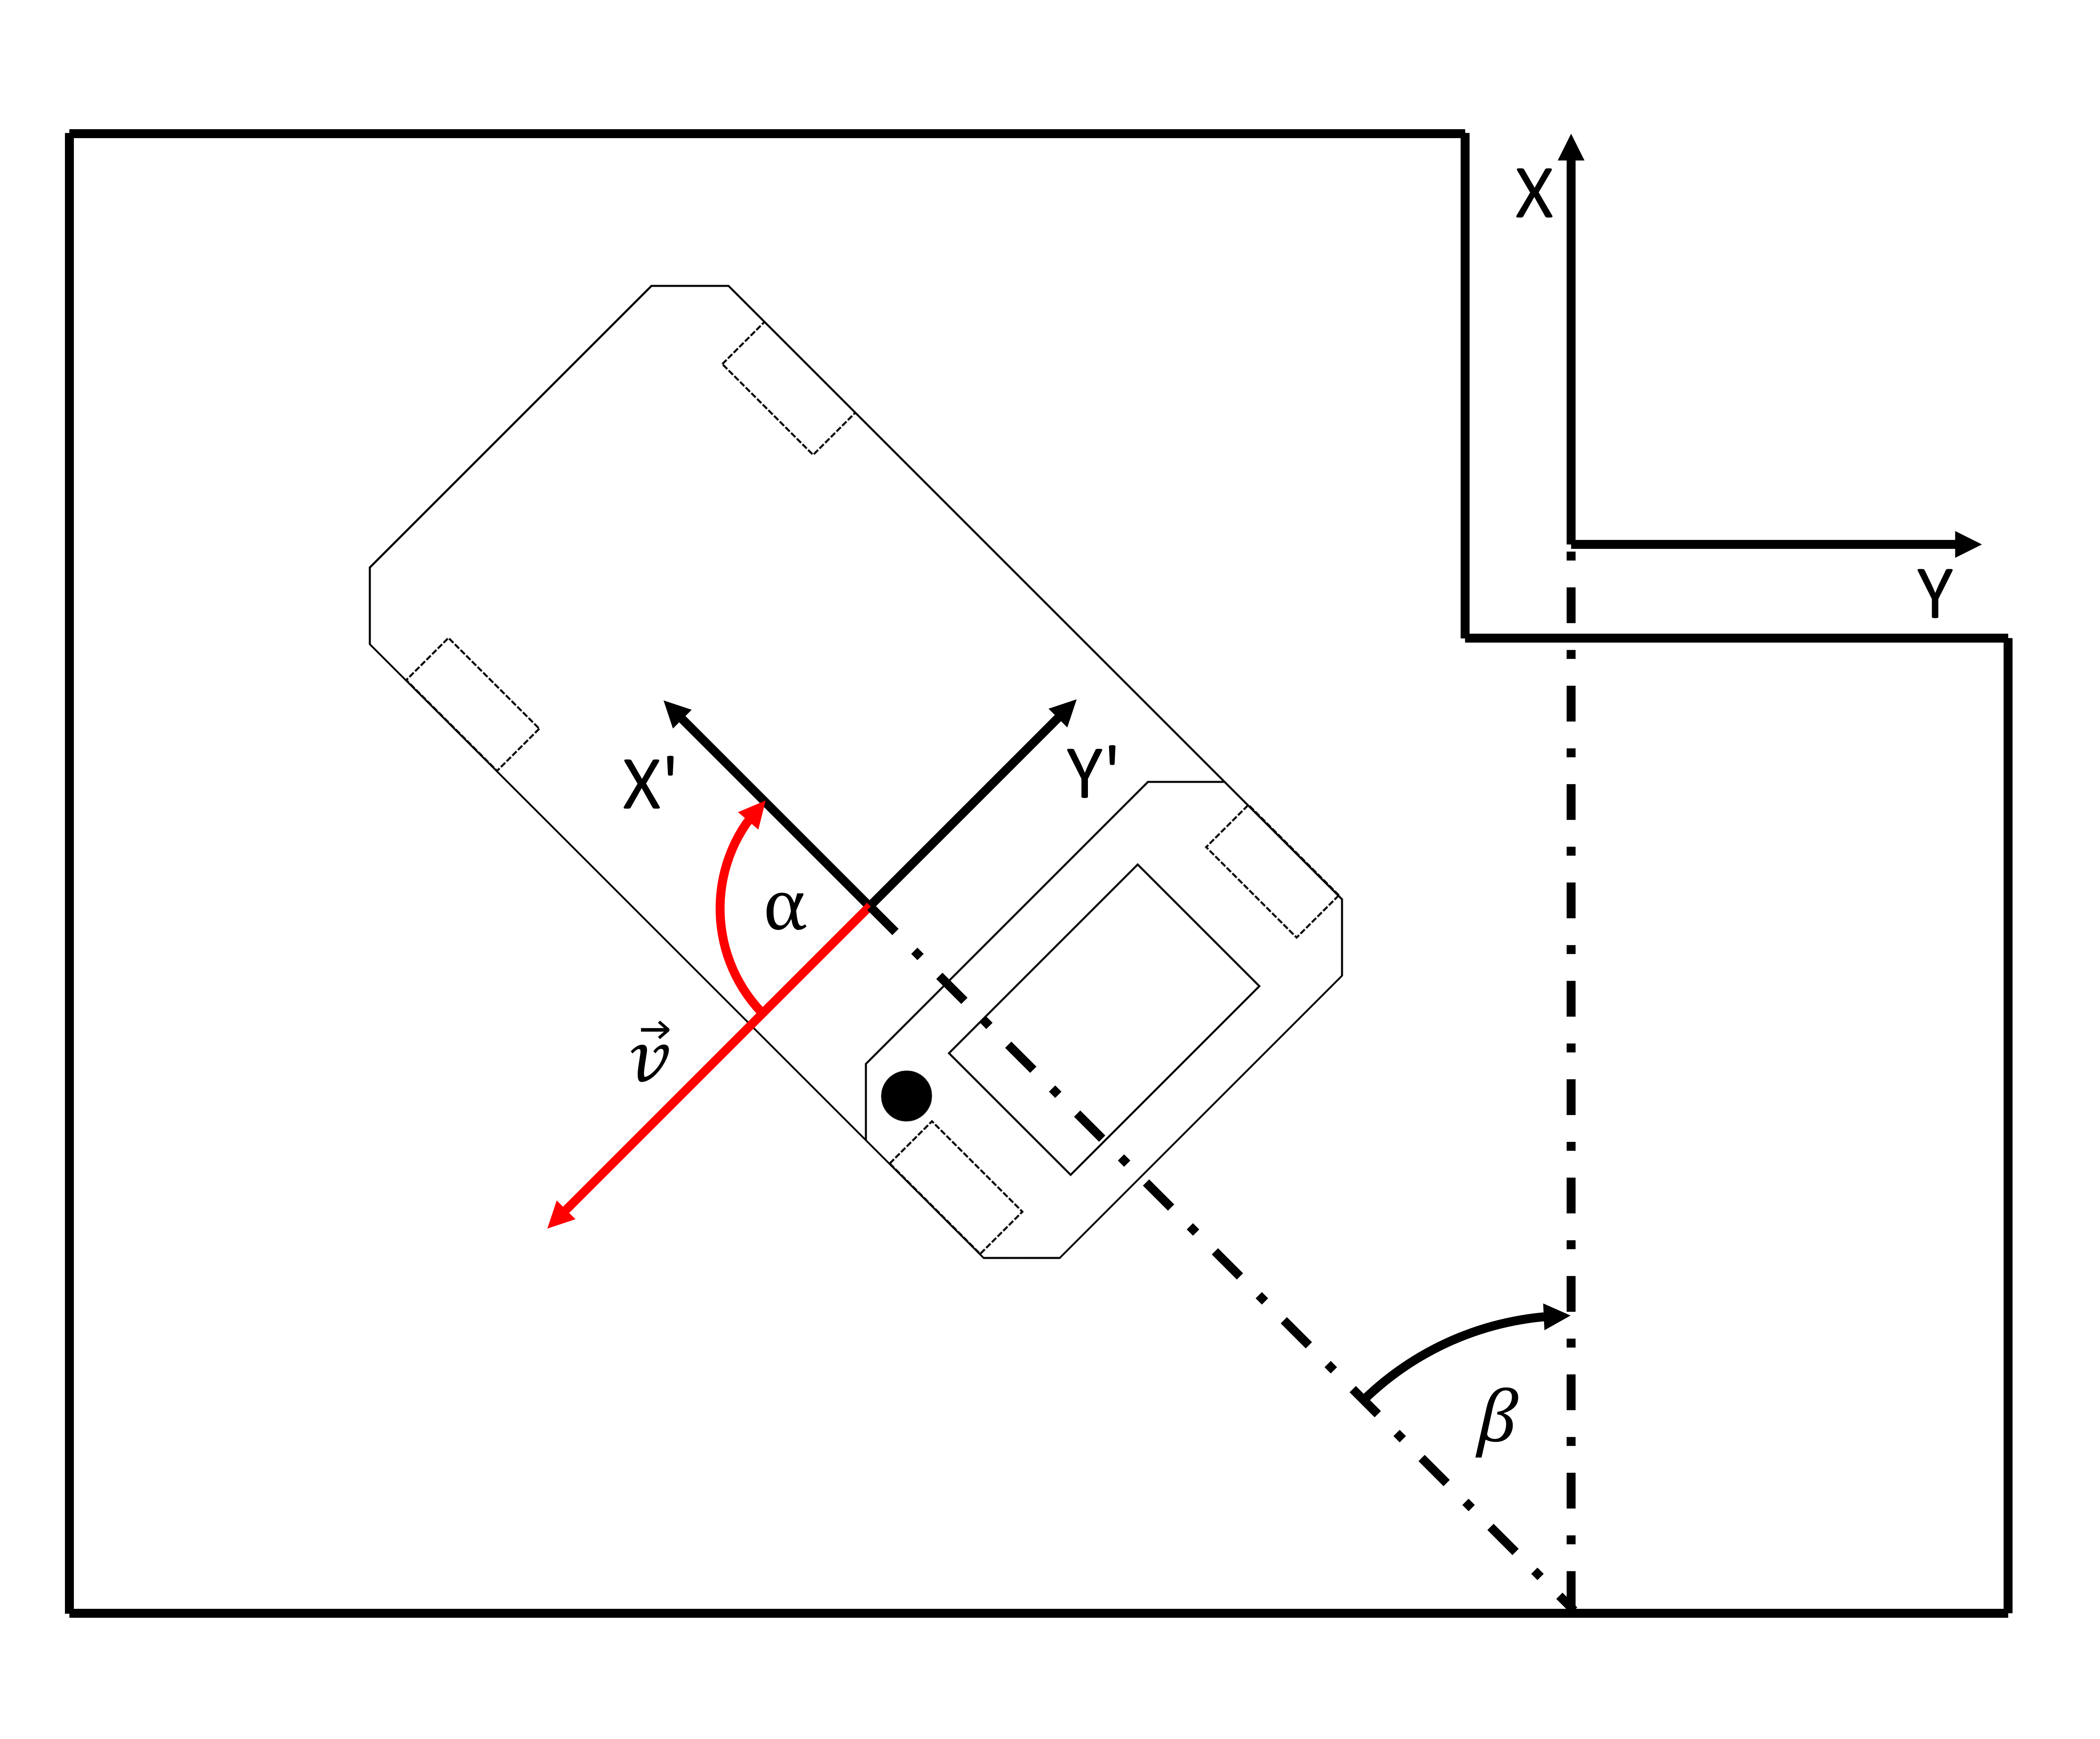
\includegraphics[width=0.8\textwidth]{Bilder/posenundfahrtwinkel.png}
			\caption{Darstellung des Posen- und Fahrtwinkels aus der Draufsicht. Im Zentrum der Abbildung ist das ALF mit dem lokalen Koordinatensystem des Fahrzeugs zu sehen. Der Fahrtwinkel $\alpha$ liegt zwischen der X-Achse des lokalen Koordinatensystems und dem als roten Pfeil dargestellten Geschwindigkeitsvektor des Fahrzeugs. Oben rechts in der Darstellung befindet sich das globale Koordinatensystem. Der Posenwinkel ist hier mit $\beta$ gekennzeichnet.}
			\label{fig: Posen- und Fahrtwinkel}
		\end{figure}
		
		Mithilfe dieser Unterteilung wird ein translatorisches Bewegungsziel mithilfe des Fahrtwinkels und ein rotatorisches durch den Posenwinkel vorgegeben. Das translatorische Bewegungsziel kann durch zwei Quellen generiert werden. Die Daten des Joysticks und die des Knotens \textit{Move Base}, der in Kapitel \ref{subsubsec: Erstellen der Bewegungsplanung} erklärt wird, können hierfür verwendet werden. Je nach Betriebsmodus werden X- und Y-Richtungskomponenten aus den Daten des Joysticks oder die des Knotens generiert. Mithilfe dieser Komponenten und des Simulinkblocks \textit{Polar to Cartesian} wird der Fahrtwinkel $\alpha$ bestimmt. Dieser wird mit einer Multiplikation des Vektors $\vec{a}$ und der Hilfsmatrix $\underline{H}$, wie in Gleichung (\ref{eq: Fahrtwinkel}) in ein translatorisches Bewegungsziel $\vec{t}_{ma}$ überführt. Die Hilfsmatrix $\underline{H}$ wird für die Umrechnung in eine in der Praxis anwendbare mathematische Form verwendet. Dessen Zeilen entsprechen jeweils einem Rad des Fahrzeugs in der Reihenfolge von oben nach unten vorne rechts, vorne links, hinten rechts und hinten links. Die Spalten enthalten die Multiplikatoren für die Komponenten in Vektor $\vec{a}$. 
		
		\begin{equation}
		\vec{t}_{ma} = \underline{H} \cdot \vec{a}
		\text{ }
		\text{ }
		\text{ mit }
		\text{ }
		\text{ }
		\underline{H}=\left(
		\begin{array}{rr}
		1&-1\\
		1&1\\
		1&1\\
		1&-1\\
		\end{array}\right)
		\text{ }
		\text{ }
		\text{ und }
		\text{ }
		\text{ }
		\vec{a}=\left(
		\begin{array}{c}
		\cos(\alpha)\\
		\sin(\alpha)\\
		\end{array}\right)
		\label{eq: Fahrtwinkel} 
		\end{equation}\\				
		Das rotatorische Bewegungsziel kann ebenfalls manuell über den Joystick oder durch den bewegungsplanenden Knoten erzeugt werden. Das durch die manuelle Steuerung erzeugte rotatorische Bewegungsziel wird als Vektor $\vec{r}_m$ gekennzeichnet. Hierbei wird der Soll-Posenwinkel durch Drücken der entsprechenden Tasten am Joystick in \textit{Simulink} inkrementiert beziehungsweise dekrementiert. Der Ist-Posenwinkel wird aus dem ROS-Knoten \textit{Hector Slam} gewonnen, der in Kapitel \ref{subsubsec: Erstellen der Bewegungsplanung} beschrieben wird. Durch eine Multiplikation der Differenz aus Soll- und Ist-Posenwinkel mit einem empirisch ermittelten Faktors $P_m$ und des Hilfsvektors $\vec{h}$ entsteht das Bewegungsziel $\vec{r}_m$ aus Gleichung (\ref{eq: rotatorisch manuell}). Der Faktor $P_m$ ist durch die Winkeldifferenz zwischen Soll- und Ist-Posenwinkel begründet. Gemäß des Anhangs \ref{it: Lastenheft} darf dieser den Wert von 10$^\circ$ nicht übersteigen. Mit der Differenz nimmt die Dominanz des rotatorischen Bewegungsziels zu beziehungsweise ab. Ab einem Wert von maximal 10$^\circ$ wird nur das rotatorische Bewegungsziel umgesetzt.
		
		\begin{equation}
		\vec{r}_m = \Delta \beta \cdot P_{m} \cdot \vec{h}
		\text{ }
		\text{ }
		\text{ mit }
		\text{ }
		\text{ }
		P_m = \frac{1}{10^\circ} 
		\text{ }
		\text{ }
		\text{ und }
		\text{ }
		\text{ }
		\vec{h} = \left(
		\begin{array}{r}
		-1\\
		1\\
		-1\\
		1\\
		\end{array}\right)
		\label{eq: rotatorisch manuell}
		\end{equation}\\
		Für die automatische Steuerung des Fahrzeugs wird mithilfe des Knotens \textit{Move Base} eine Trajektorie geplant. Die Gewinnung einer solchen Trajektorie wird in Kapitel \ref{subsubsec: Erstellen der Bewegungsplanung} erläutert. Aus dem Topic \textit{cmd\_vel} lässt sich ein rotatorischer Bewegungsbefehl $c$ für die Verfolgung einer Trajektorie auslesen. Analog zur Winkeldifferenz wird dieser Wert mit einem empirisch ermittelten Faktor $P_{a}$ skaliert und mit einem Hilfsvektor $\vec{h}$ multipliziert. Das Ergebnis ist das daraus folgende Bewegungsziel $\vec{r}_{a}$ und wird in Gleichung (\ref{eq: rotatorisch auto}) gezeigt. Der Betrag des Faktors $P_a$ wurde nach dem Rotationsbefehl aus dem Topic \textit{cmd\_vel} ausgelegt, der in Kapitel \ref{subsec: Bewegungsbefehle} erläutert wird. In den Parametern des Topics ist für den Rotationsbefehl ein Höchstwert von 0,5 hinterlegt. Aus der Dokumentation des entsprechenden Knotens ist nicht ersichtlich, wann der Höchstwert eintritt \cite{teblp}. Fordert das Topic diesen Wert als rotatorischen Bewegungsbefehl $c$, wird es aufgrund des Faktors $P_a$ vorrangig abgearbeitet. 
						
		\begin{equation}
		\vec{r}_a = c \cdot P_{a} \cdot \vec{h}
		\text{ }
		\text{ }
		\text{ mit }
		\text{ }
		\text{ }
		P_a = -2 
		\text{ }
		\text{ }
		\text{ und }
		\text{ }
		\text{ }
		\vec{h} = \left(
		\begin{array}{rr}
		-1\\
		1\\
		-1\\
		1\\
		\end{array}\right)
		\label{eq: rotatorisch auto}
		\end{equation}\\
		Die drei Ziele können rechnerisch durch eine Addition der Vektoren vereint werden und ergeben ein neues, gemeinsames Bewegungsziel $\vec{b}$. 
		
		\begin{equation}
		\vec{t}_{ma} + \vec{r}_m + \vec{r}_a = \vec{b} 
		\label{eq: posenfahrt}
		\end{equation}  \\		
		Wird der Vektor des resultierende Bewegungsziel $\vec{b}$ mit der geforderten Drehzahl multipliziert erhält man die Soll-Drehzahl aller Räder. Diese werden in der Drehzahlregelung, wie in Kapitel \ref{sec: Drehzahlregelung} beschrieben, als Eingangsgröße verwendet.  
		
		\begin{figure}[H]
			\centering
			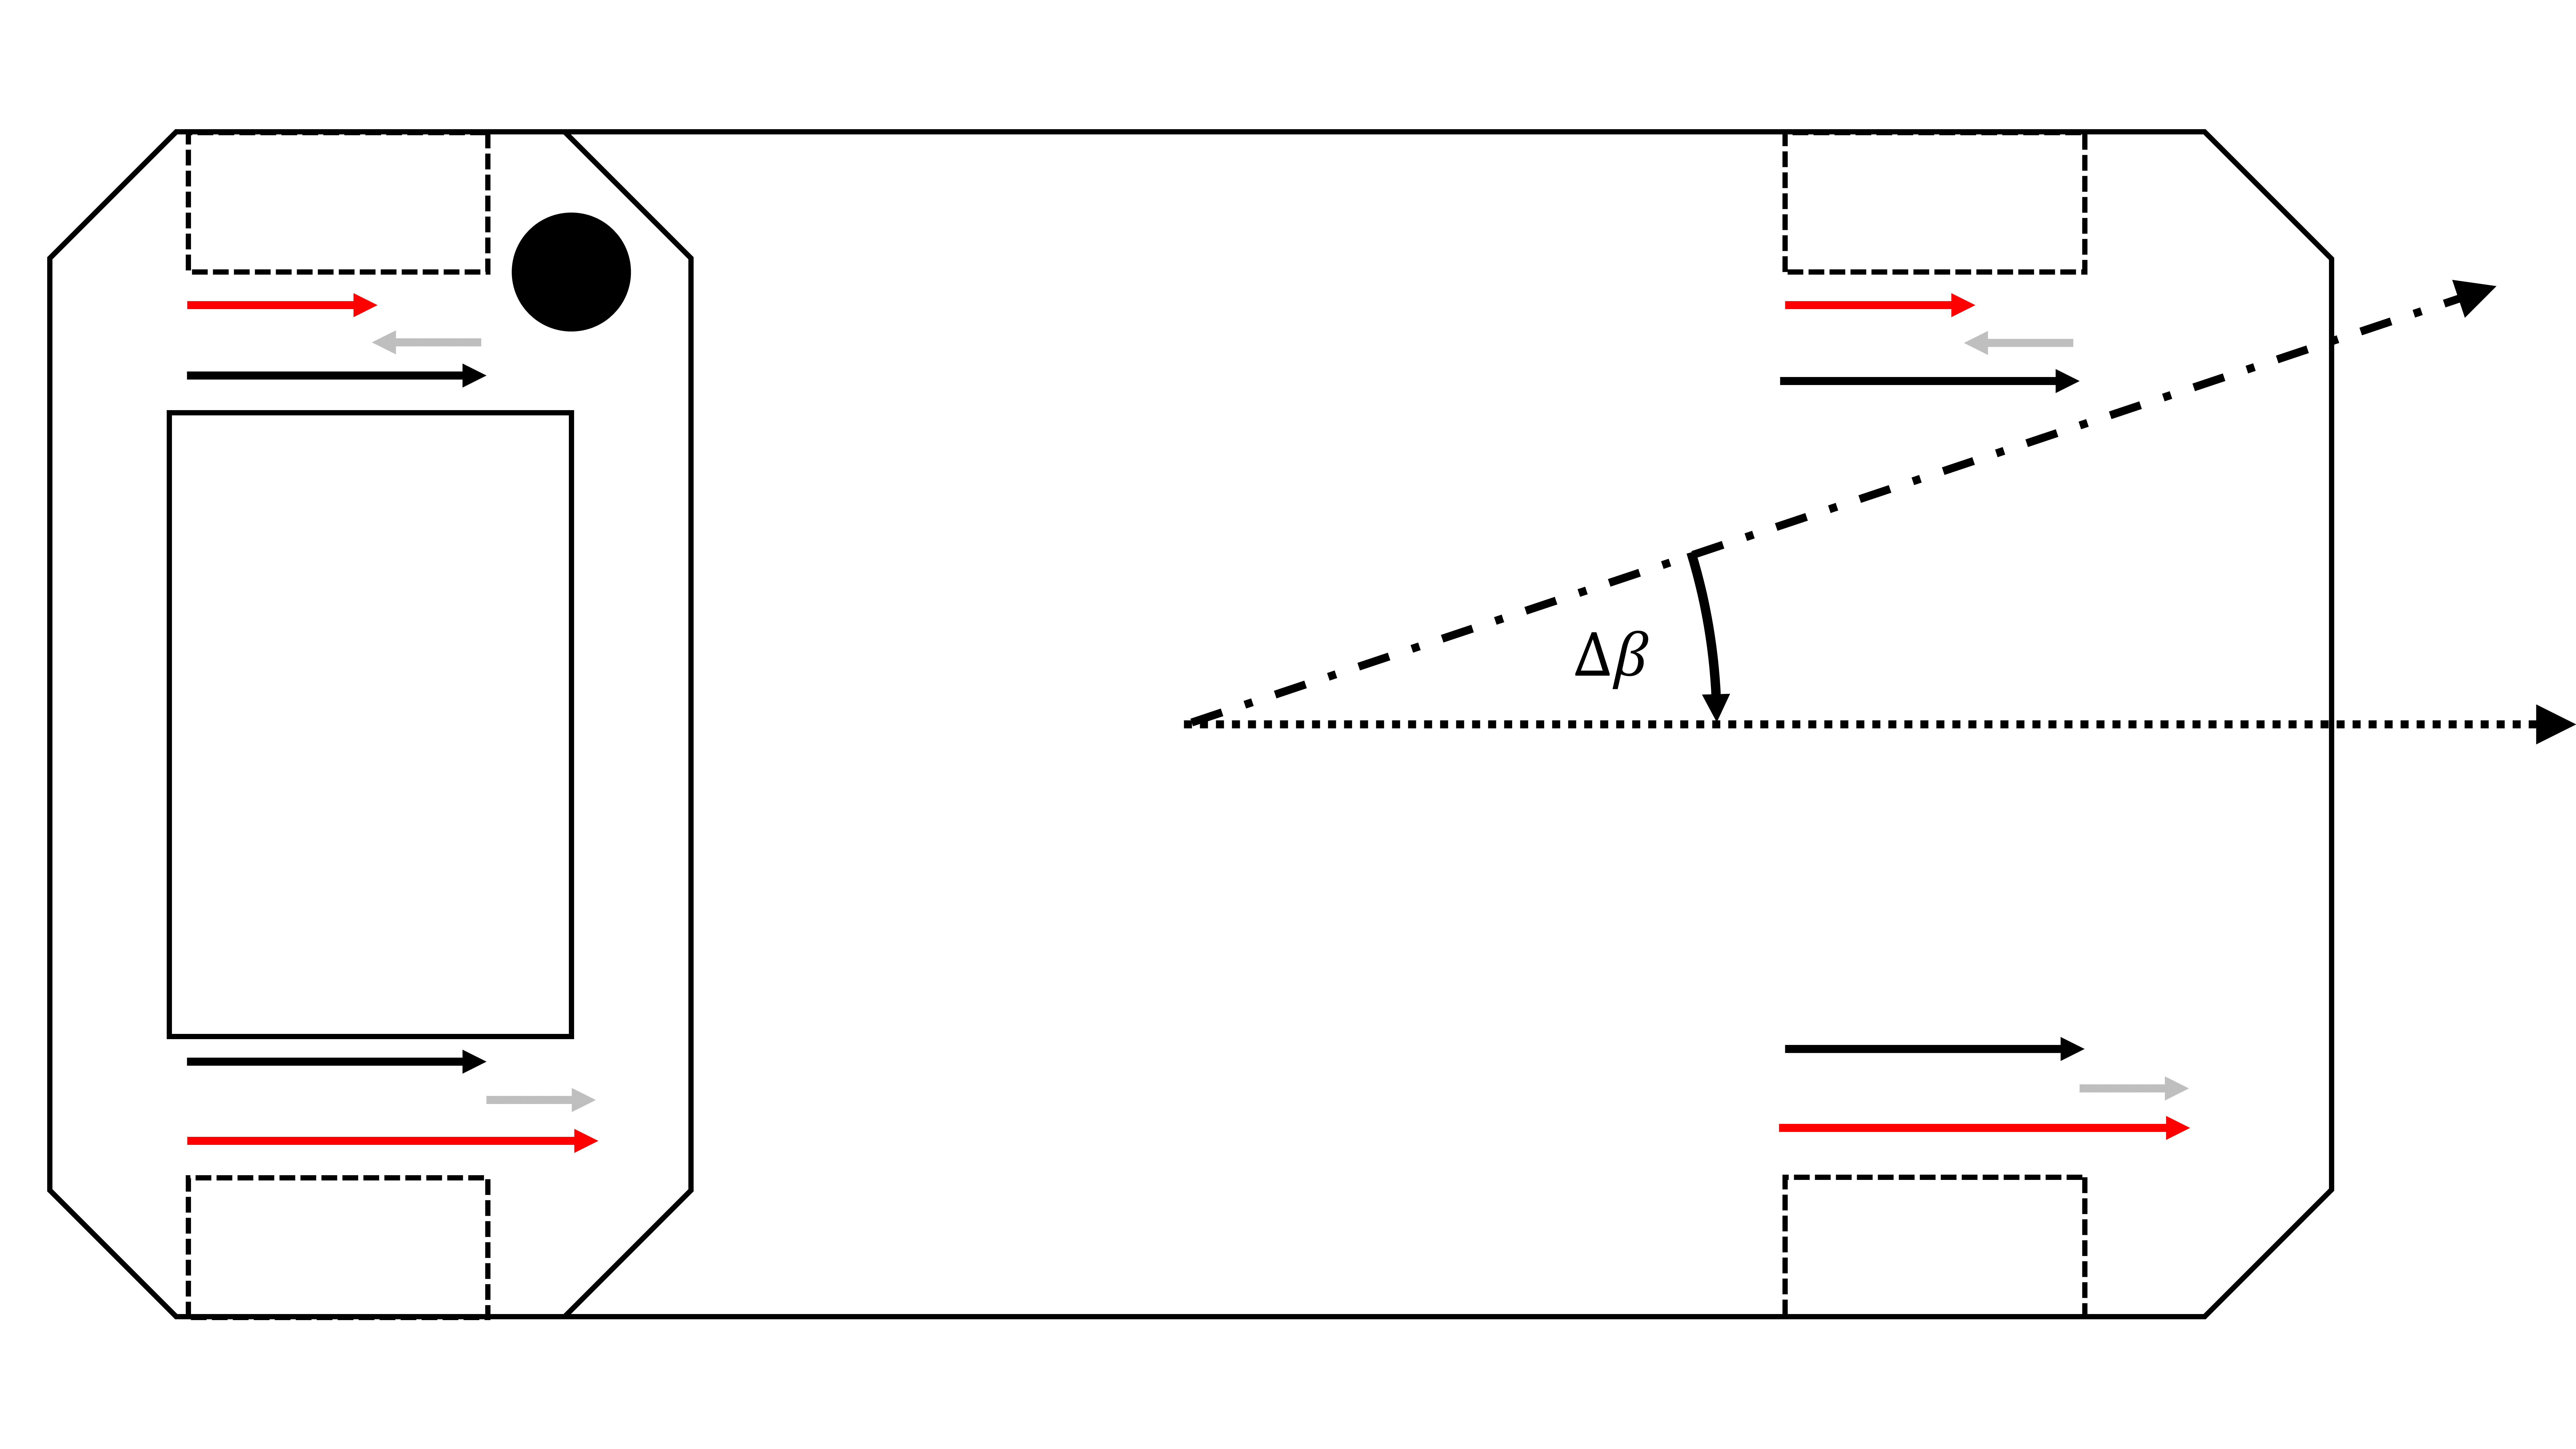
\includegraphics[width=1.0\textwidth]{Bilder/winkelregelung.png}
			\caption{Darstellung des Funktionsprinzips der Lageregelung aus der Draufsicht des ALFs. Der schwarze, gepunktete Vektor zeigt die momentane Ausrichtung der Pose. Der als Strichpunktlinie ausgeführte Pfeil ist als zu erreichende Pose zu deuten. Der dargestellte Winkel $\delta \beta$ zeigt die Posenwinkeldifferenz. Die gestrichelten Vierecke in den Ecken des Fahrzeugs stellen die Räder dar. Für jedes Rad sind Pfeile in die Abbildung eingetragen, die jeweils symbolisch eine Winkelgeschwindigkeit der entsprechenden Räder repräsentieren. Die schwarzen Pfeile stellen das translatorische Bewegungsziel und die grauen ein rotatorisches dar. Resultierend aus Gleichung (\ref{eq: posenfahrt}) beschreiben die roten Pfeile die Einträge des Vektors $\vec{b}$.}
			\label{fig: Winkelregelung}
		\end{figure}
		
		In Abbildung \ref{fig: Winkelregelung} ist die Funktionsweise der Lageregelung prinzipiell dargestellt. Das Fahrzeug soll sich hier beispielhaft mit einem Fahrtwinkel von 0$^\circ$ entlang des grünes Pfeils, der als Strichpunktlinie dargestellt ist, ausrichten und geradeaus fahren. Der rote, als Strichpunktlinie dargestellte Pfeil zeigt die momentane Ausrichtung der Pose. Der Winkel $\delta \beta$ zeigt die Differenz zwischen Soll- und Ist-Pose. Die schwarzen Pfeile stellen den Betrag und die Richtung der Einträge des aus den Fahrtwinkel errechneten Vektors dar. Der Posenwinkel wird in diesem Beispiel verändert und erzeugt einen Vektor der hier mit roten Pfeilen symbolisch gezeigt wird. Nach der Berechnung nach Gleichung (\ref{eq: posenfahrt}) ergibt sich der resultierende Vektor $\vec{b}$, dessen Einträge in Abbildung \ref{fig: Winkelregelung} durch grüne Pfeile dargestellt werden. 
		
				
			


		\section{Auswertung der Sensordaten}
		\label{subsec: Auswerten der Sensordaten}
		
			Die Verarbeitung der Sensorsignale ist für eine kollisionsfreie Bewegung des Fahrzeugs im automatischen Betrieb notwendig. Neben der Visualisierung dieser Signale ist im Folgenden die Integration in das System beschrieben.
		
			\subsection{Visualisierung der Sensordaten}
			\label{subsubsec: Visualisierung der Sensordaten}
			
			ROS Visualization, oder auch Rviz genannt, ist ein 3D-Visualisierungstool und wird für die Anzeige von Sensordaten und Statusinformationen genutzt. Zur Visualisierung des Robotermodels in \textit{Rviz}, wird eine \textit{Unified Robot Description Format} (URDF) Datei erstellt \cite{urdf}. In der URDF Datei werden vom Benutzer dreidimensionale Körper programmiert und ausgerichtet. In Abbildung \ref{fig: URDF} ist das mit der URDF-Datei erzeugte und in \textit{Rviz} visualisierte ALF zu sehen.
			
			\begin{figure}[H]
				\centering
				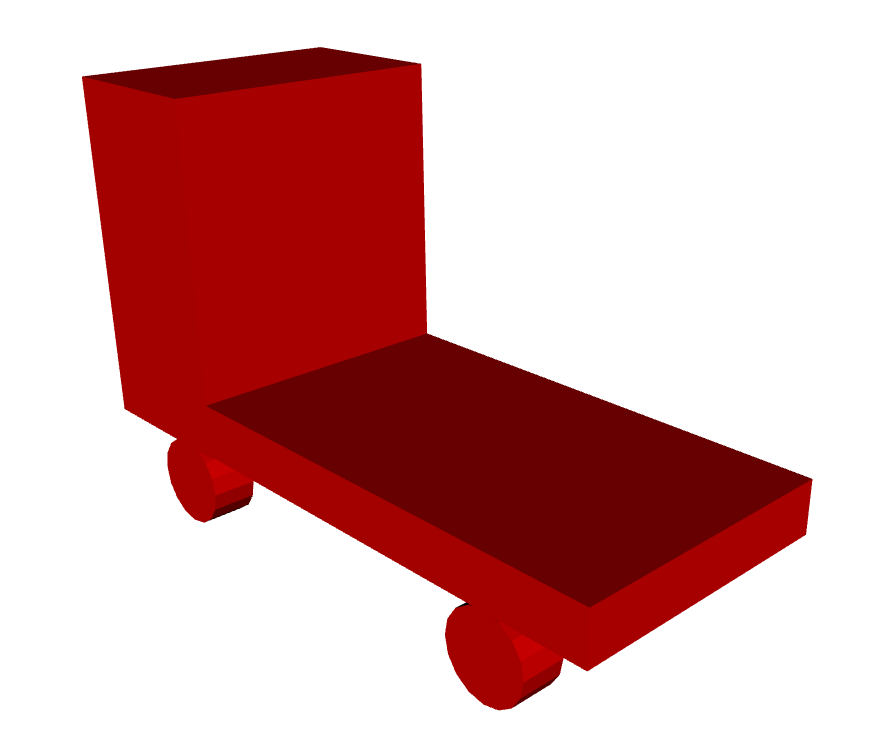
\includegraphics[width=0.6\textwidth]{Bilder/urdf.png}
				\caption{Visualisierung des in Rviz importierten Robotermodells von schräg oben betrachtet.}
				\label{fig: URDF}
			\end{figure}
			
			Wenn der Knoten Rviz gestartet wird öffnet sich eine Benutzeroberfläche auf der die entsprechenden Topics abonniert werden können. Für eine bessere Übersicht lassen sich die visualisierten Sensordaten einfärben, um diese später voneinander unterscheiden zu können. Ebenfalls ist es möglich in Rviz eine 2D-Pose einzugeben, die als Navigationsziel für den in Kapitel \ref{subsec: Kartografierung und Bewegungsplanung} erklärten Trajektorie Planer dient. \cite{rviz}  
		
		    \subsection{Einbindung des RPLIDAR A2}
		    \label{subsubsec: Übersetzen der Laserdaten}
		    	
		    	Die Integration der Messwerte des \textit{RPLIDAR A2} in das ROS-Netzwerk wird durch den Knoten \textit{Rplidar} umgesetzt \cite{lidar}. Bei dem Aufruf des Knotens wird der Motor des $360^\circ$-Laserscanners gestartet und das Topic \textit{Scan} mit dem Nachrichtentyp \textit{LaserScan} veröffentlicht \cite{lidar}. In Abbildung \ref{fig: Laserscan des RPLIDAR in Rviz} sind Beobachtungen von Landmarken des Lidar-Sensors als schwarze Punkte zu sehen.
		    	
		    	\begin{figure}[H]
		    		\centering
		    		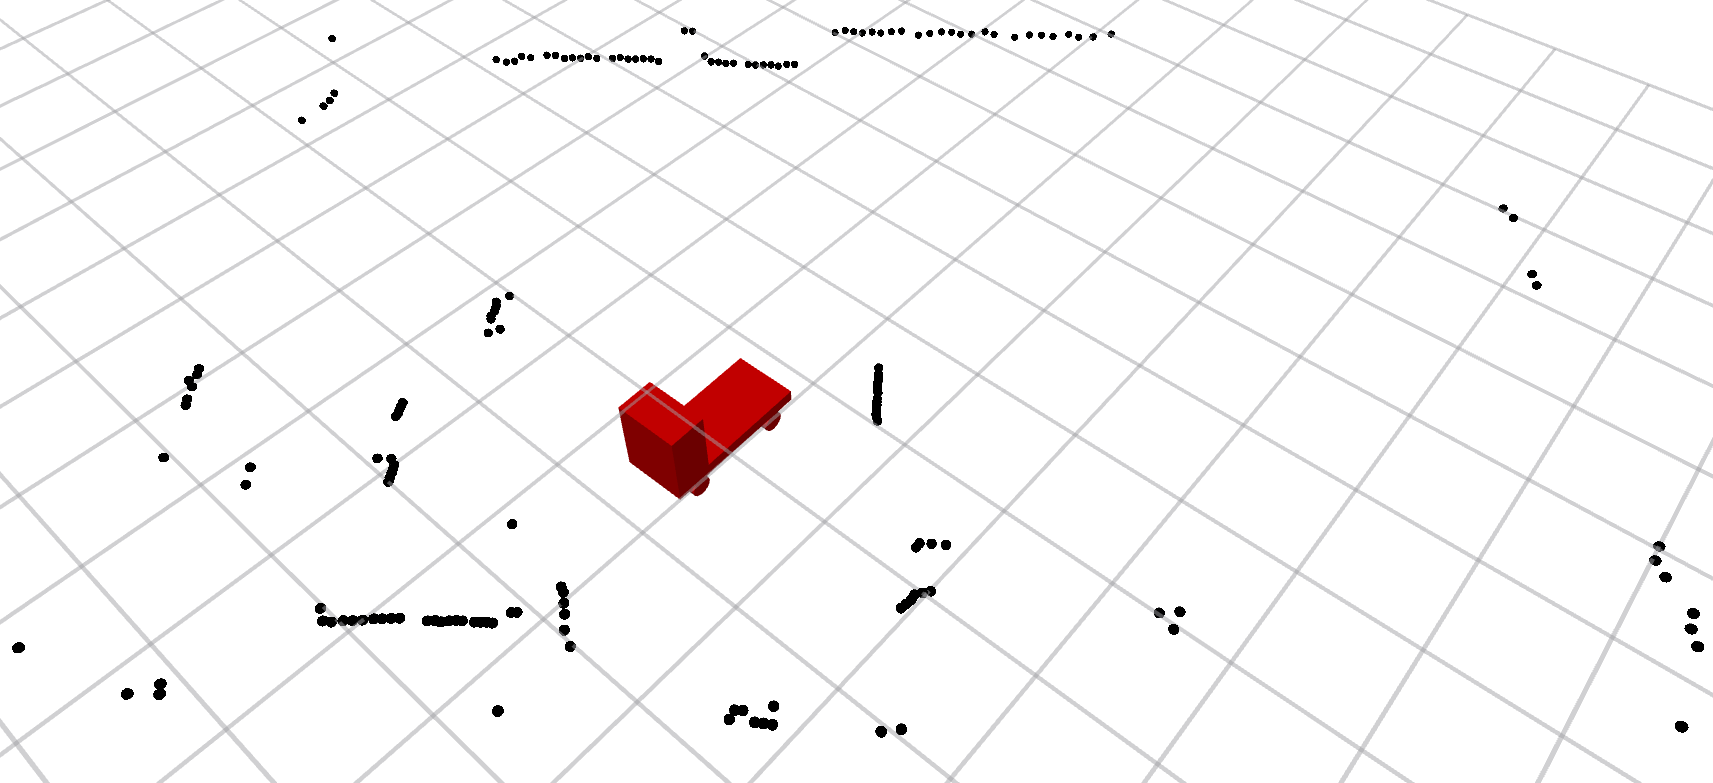
\includegraphics[width=1.0\textwidth]{Bilder/laserscan.png}
		    		\caption{Die Abbildung zeigt die in \textit{Rviz} visualisierten Sensorsignale des \textit{RPLIDAR A2}. Die schwarzen Punkte stellen die von dem Lidar-Sensor veröffentlichten Daten dar und repräsentieren die von diesem erkannten Objekte. Mittig in der Darstellung ist das durch die URDF-Datei importierte, rote Robotermodell zu sehen. }
		    		\label{fig: Laserscan des RPLIDAR in Rviz}
		    	\end{figure}
		    
		    	
		    \subsection{Integration der Kinect-Sensoren}
		    \label{subsubsec: Kinect-Sensor}	    
		    
		    	Für die Implementieren der von den \textit{Kinect}-Sensoren aufgenommenen Bildinformationen in das ROS-Netzwerk wird in dieser Bachelorarbeit der Knoten \glqq Kinect2 Bridge\grqq{} benutzt. Das Softwarepaket enthält eine Kalibrierung, eine Registrierung, ein eigenständiges Anzeigewerkzeug für das Kamerabild und einige Knoten für die Veröffentlichung aller Kamerafunktionen als Topic. 
		    	
		    	Um Softwareabstürze zu vermeiden, die bei der Inbetriebnahme von zwei \textit{Kinect}-Sensoren auftreten, wird der Buffer des \textit{Universal Serial Bus Filesystem} (USBFS) vergrößert \cite{libfreenect2troubleshooting}.
		    	Zudem wird die Bildrate auf maximal 5 Bilder pro Sekunde reduziert, anschließend konnten beide \textit{Kinect}-Sensoren ohne Probleme betrieben werden. \cite{iaikinect}\\
		   		    
		    	Das vom Knoten \textit{Kinect2 Bridge} veröffentlichte Topic \textit{kinect2/hd/image\_depth\_rect} ist vom Nachrichtentyp \textit{Image}. Dieses kann von dem in Kapitel \ref{subsubsec: Erstellen der Bewegungsplanung} beschriebenen Knoten \textit{Move Base} nicht verwendet werden, da Nachrichten von dem Typ \textit{LaserScan} benötigt werden.
			    Deshalb wird der Knoten \textit{Depthimage To Laserscan} benutzt, um eine Typkonvertierung von \textit{Image} zu \textit{LaserScan} durchzuführen.
		    	Ein relevanter Parameter für die Typkonvertierung ist \textit{scan\_height}, der die genutzte Anzahl der horizontal angelegten Pixelreihen des Bildes beschreibt. Der Knoten ermittelt spaltenweise den kleinsten gemessenen Abstand und veröffentlicht diesen Wert mit dem Nachrichttyp \textit{LaserScan}.
		    	Als Ergebnis der Typkonvertierung können die \textit{Kinect}-Sensoren für die Navigation als Observierungsquelle genutzt werden.
		    	Im Rahmen dieser Bachelorarbeit werden die konvertierten Nachrichten des Typs \textit{LaserScan} in den Topics \textit{Scan1} und \textit{Scan2} von den Knoten der beiden \textit{Kinect}-Sensoren veröffentlicht. \cite{depthimagetolaserscan}
		    	
		   
		     	\begin{figure}[H]
		     		\centering
		     		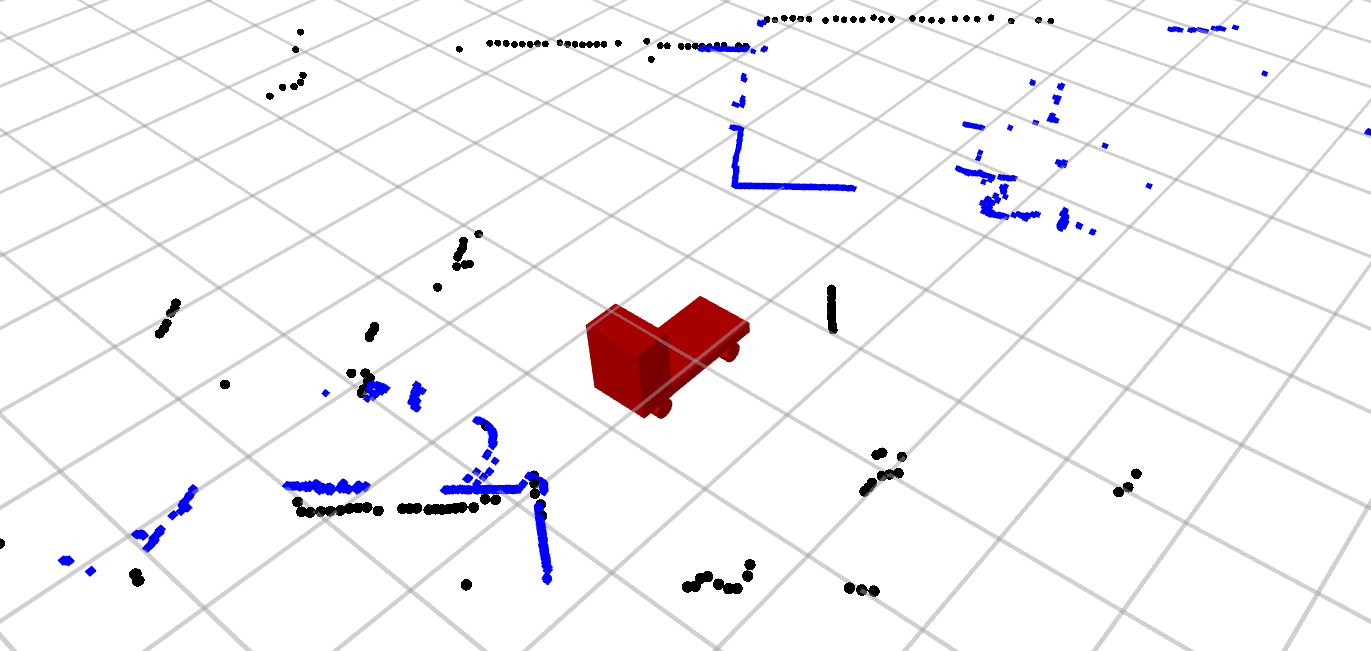
\includegraphics[width=1.0\textwidth]{Bilder/lidarundkinect.png}
		     		\caption{Darstellung der Sensorsignale in \textit{Rviz} von schräg oben betrachtet. Im Zentrum der Abbildung ist das ALF als Modell dargestellt. Die schwarzen Markierungen sind von \textit{Rviz} abonnierte und visualisierte Sensorsignale des \textit{RPLIDAR A2}. Die blauen Punkte sind Daten der \textit{Kinect}-Sensoren. Die Markierungen stellen von den Sensoren erkannte Objekte dar.}
		     		\label{fig: Laserscans in Rviz}
		     	\end{figure}
		     	
		     	In Abbildung \ref{fig: Laserscans in Rviz} sind die Sensorsignale des Lidar-Sensors als schwarze und der beiden \textit{Kinect}-Sensoren als blaue Punkte dargestellt. Oben rechts und unten links in der Abbildung ist zu erkennen, dass die Sensordaten teilweise nicht korrelieren. Dies ist auf die \textit{Kinect}-Sensoren zurückzuführen, da Objekte unter der Arbeitshöhe des 360$^\circ$-Laserscanners liegen erkannt werden. In der Darstellung \ref{fig: Verifikation der erfassten Laserdaten} können die in Abbildung \ref{fig: Laserscans in Rviz} gezeigten Laserdaten nachvollzogen und realen Objekten zugeordnet werden.
		     	
		     %	Dies bedeutet nicht, dass fehlerhafte Daten vorliegen oder die Koordinatentransformation falsch durchgeführt wurde sondern dass Objekte, die unter die Arbeitshöhe des 360$^\circ$-Laserscanners fallen von den Kinect-Sensoren erfasst werden.
		     	
		     	\begin{figure}[H]
		     		\centering
		     		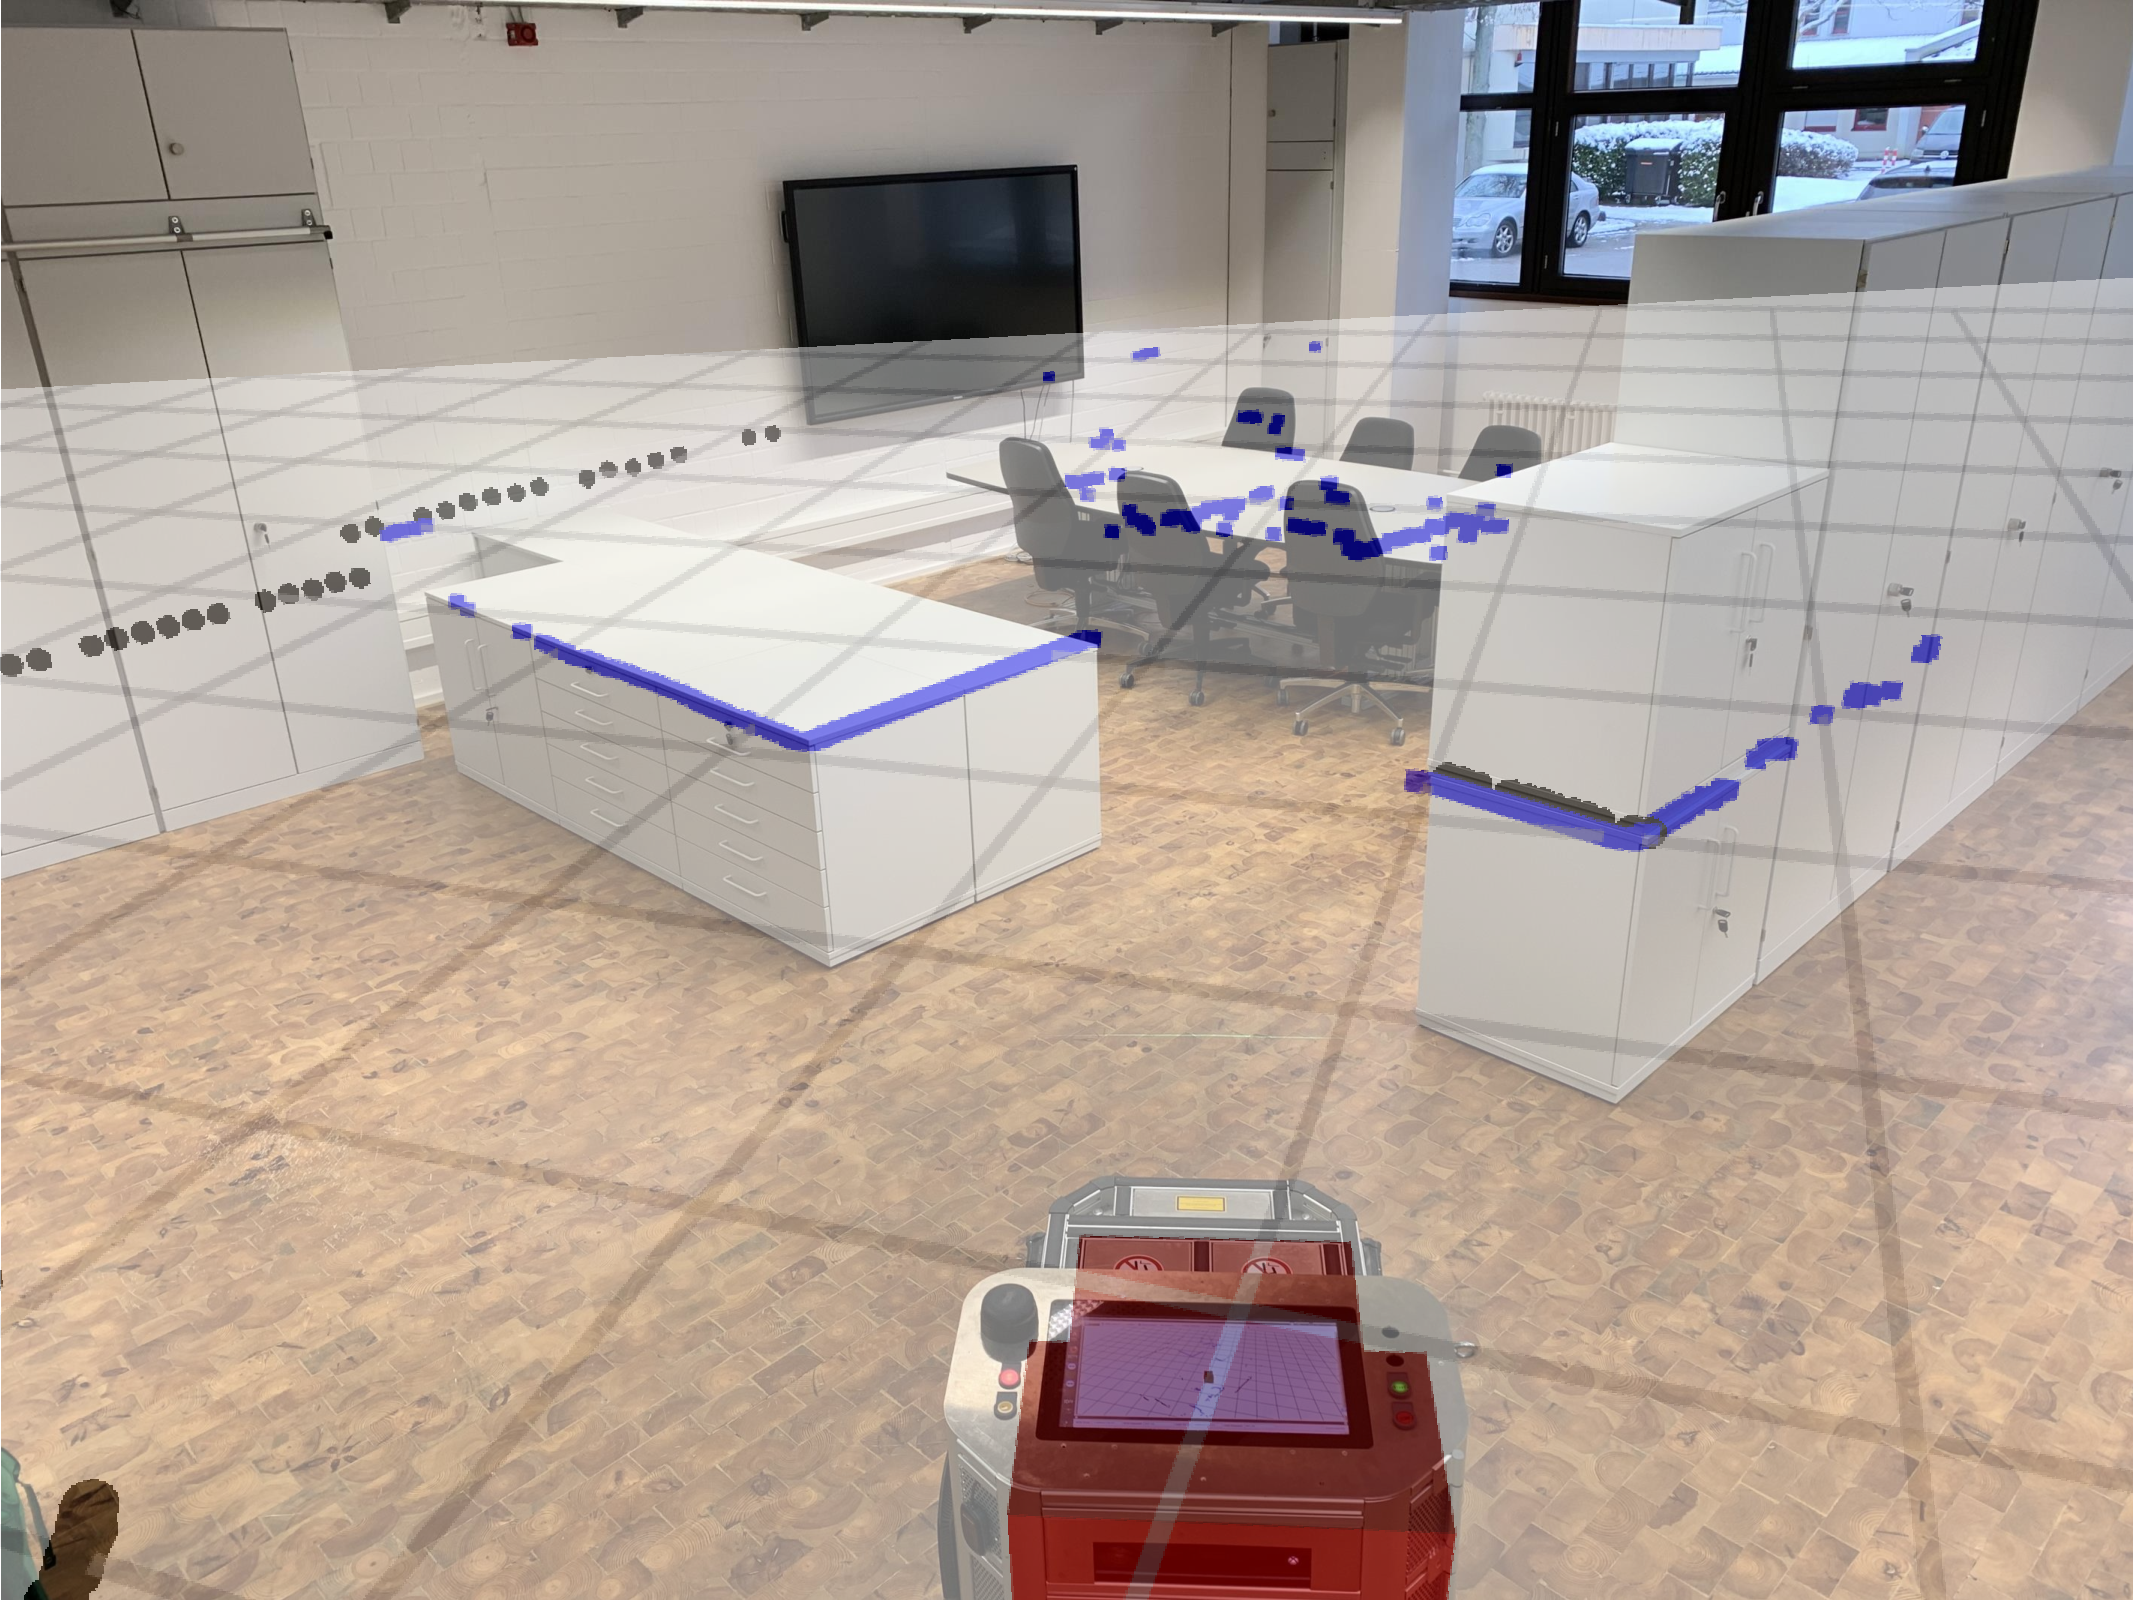
\includegraphics[width=1.0\textwidth]{Bilder/match.pdf}
		     		\caption{Visualisierung der \textit{LaserScan}-Topics aus den Kapiteln \ref{subsubsec: Übersetzen der Laserdaten} und \ref{subsubsec: Kinect-Sensor} in \textit{Rviz}. Zeich it ein Foto aus gleicher Perspektive unter das Bildschirmfoto aus \textit{Rviz} gelegt. Die erfassten Gegenstände der \textit{Kinect}-Sensoren sind in diesem Fall als blaue Markierungen und die des \textit{RPLIDAR A2} als schwarz dargestellt. Die \textit{Kinect}-Sensoren erkennen im Zentrum der Darstellung einen Schrank, der von dem \textit{RPLIDAR A2} Sensor nicht erfasst wird. In Kapitel \ref{subsec: Kartografierung und Bewegungsplanung} wird auf die Folgen dieser Beobachtung eingegangen.}
		     		\label{fig: Verifikation der erfassten Laserdaten}
		     	\end{figure}
		     	
%		     \subsection{Anbindung der Fernsteuerung}
%		     \label{subsubsec: Anbindung des Xbox-Controllers}
%		     
%		     \begin{figure}[H]
%		     	\centering
%		     	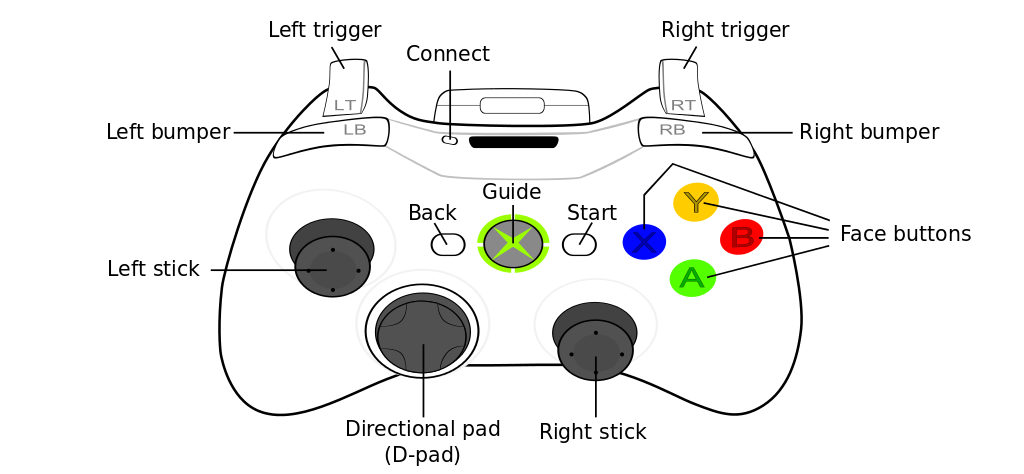
\includegraphics[width=0.8\textwidth]{Bilder/xboxcontroller.png}
%		     	\caption{Layout des XBox 360 Controllers}
%		     	\label{fig: Layout des XBox 360 Controllers}
%		     \end{figure} 
%		     
%		     	Der Knoten Joy ist für die Konvertierung der vom Benutzer eingegebenen, mechanischen Signale am Joystick zu nutzbaren digitalen Signalen zuständig. Die Betätigung der Knöpfe, wie beispielsweise den farblichen auf der rechten Seite des in Abbildung \ref{fig:  Layout des XBox 360 Controllers} gezeigten Controllers, wird in ein binären Signal umgewandelt. Bei den Joysticks und Triggern werden je nach Lage Zahlenwerte zwischen -1 und 1 in das Topic \textit{Joy} veröffentlicht. \cite{joy}
		     
		\section{Kartografierung der Umgebung}
		    \label{subsec: Kartografierung und Bewegungsplanung}
		        
		        Das Lastenheft \ref{it: Lastenheft} sieht vor die Umgebung des ALFs mit und ohne eine Bewegungsvorgabe des Benutzers zu kartographieren. In diesem Kapitel werden die für die Umsetzung nötigen Schritte dargelegt.\\
		    	
		    	Zur Kartographierung der Umgebung wird in dieser Bachelorarbeit der Knoten \textit{Hector Slam} verwendet.
		   		Dieser abonniert standardmäßig die in den Kapitel \ref{subsubsec: Übersetzen der Laserdaten} beschriebene \textit{LaserScan}-Nachrichten aus dem Topic \textit{Scan} und veröffentlicht eine Karte in das Topic \textit{Map} vom Nachrichtentyp \textit{OccupanyGrid}. Diese kann in \textit{Rviz}, wie in Abbildung \ref{fig: Hector}, visualisiert oder als Bilddatei exportiert werden. Die Karte erweitert sich durch Bewegungen des ALFs. Der Knoten löst die SLAM Problematik aus Abschnitt \ref{subsec: Mathematische Beschreibung des SLAM Problems} mit den Umgebungsdaten des \textit{RPLIDAR A2} ohne Odometrieinformationen zu benötigen. \cite{hectorslam}\\
		   				   		
		   		Die hier verwendeten Observationsquellen erfassen unterschiedliche Messwerte. Dies ist nicht auf eine fehlerhafte Messung zurückzuführen sondern auf den in Kapitel \ref{sec: Sensoren zur Erkennung der Umgebung} beschriebenen Arbeitsbereich. Das Veröffentlichen von mehreren Observationsquellen in ein Topic führt unter diesen Umständen zu Komplikationen mit dem verwendeten Algorithmus.
		   		
		   		
		   		\begin{figure}[H]
		   			\centering
		   			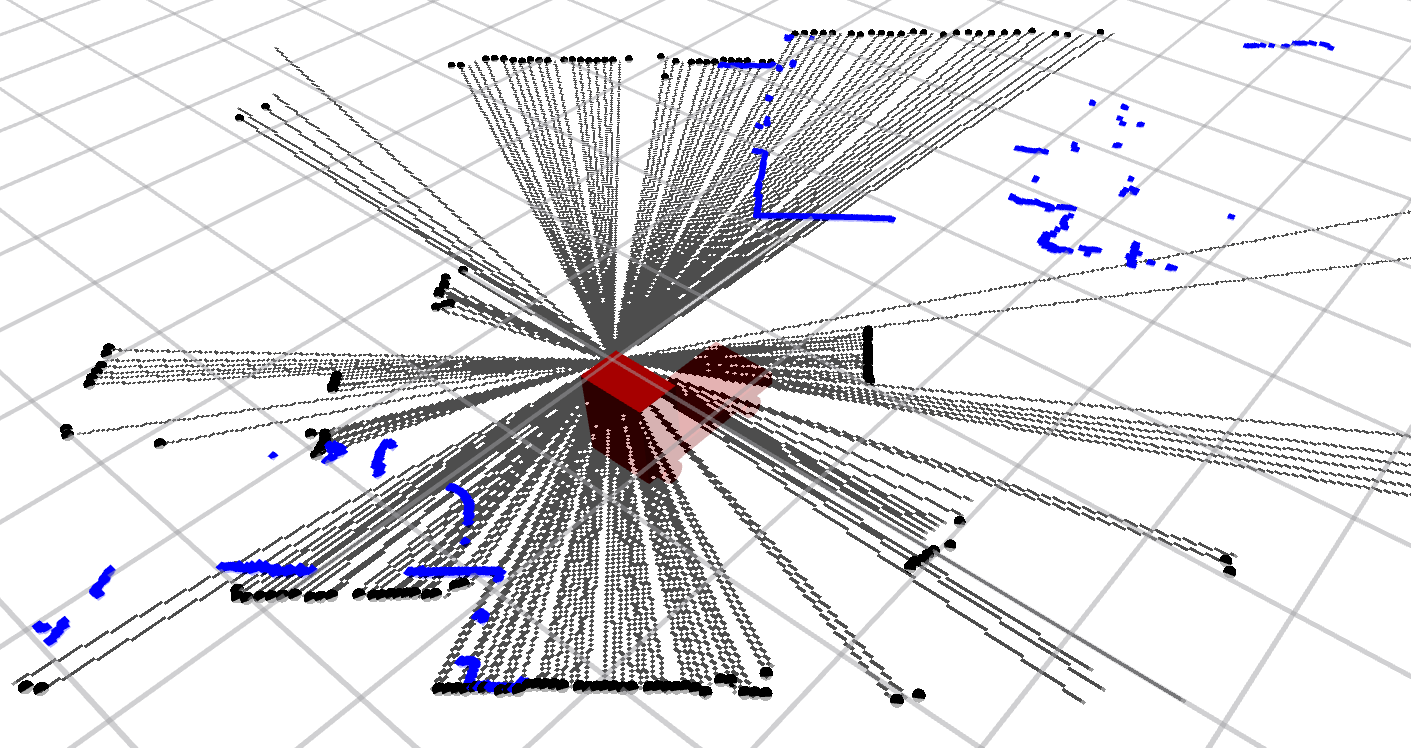
\includegraphics[width=1.0\textwidth]{Bilder/hector}
		   			\caption{Abbildung einer in Rviz dargestellten \textit{Occupancy Grid}-Karte aus dem Topic \textit{Map} und der \textit{LaserScan} Nachrichten aus Kapitel \ref{subsubsec: Übersetzen der Laserdaten} und \ref{subsubsec: Kinect-Sensor}. Zu sehen ist der Kartographierungsprozess aus der Vogelperspektive. Die schwarzen Punkte repräsentieren \textit{LaserScan} Daten des \textit{RPLIDAR A2} und die blauen der \textit{Kinect}-Sensoren. Die grauen Linien enden an einer als belegt markierten Zelle und stellen die Karte dar, die sich bei Bewegung des ALFs vervollständigt. Für die Kartographierung in der Abbildung wurden lediglich Messwerte des \textit{RPLIDAR A2} genutzt. }
		   			\label{fig: Hector}
		   		\end{figure}
		   		
		   		Desweiteren veröffentlicht der Knoten das Topic \textit{slam out pose} des Nachrichtentyps \textit{Pose} mit einer Schätzung der aktuellen Roboterposition. In diesem Nachrichtentyp wird die Orientierung des Roboters durch ein Quaternion beschrieben. Für die Verwendung des Knotens \textit{Hector Slam} ist es notwendig einen Baum aus statischen Koordinatentransformationen zu erstellen, der die Positionen aller Sensoren relativ zur geschätzten Roboterpose enthält. \cite{hectorslam}
		   		
		   		\begin{figure}[H]
		   			\centering
		   			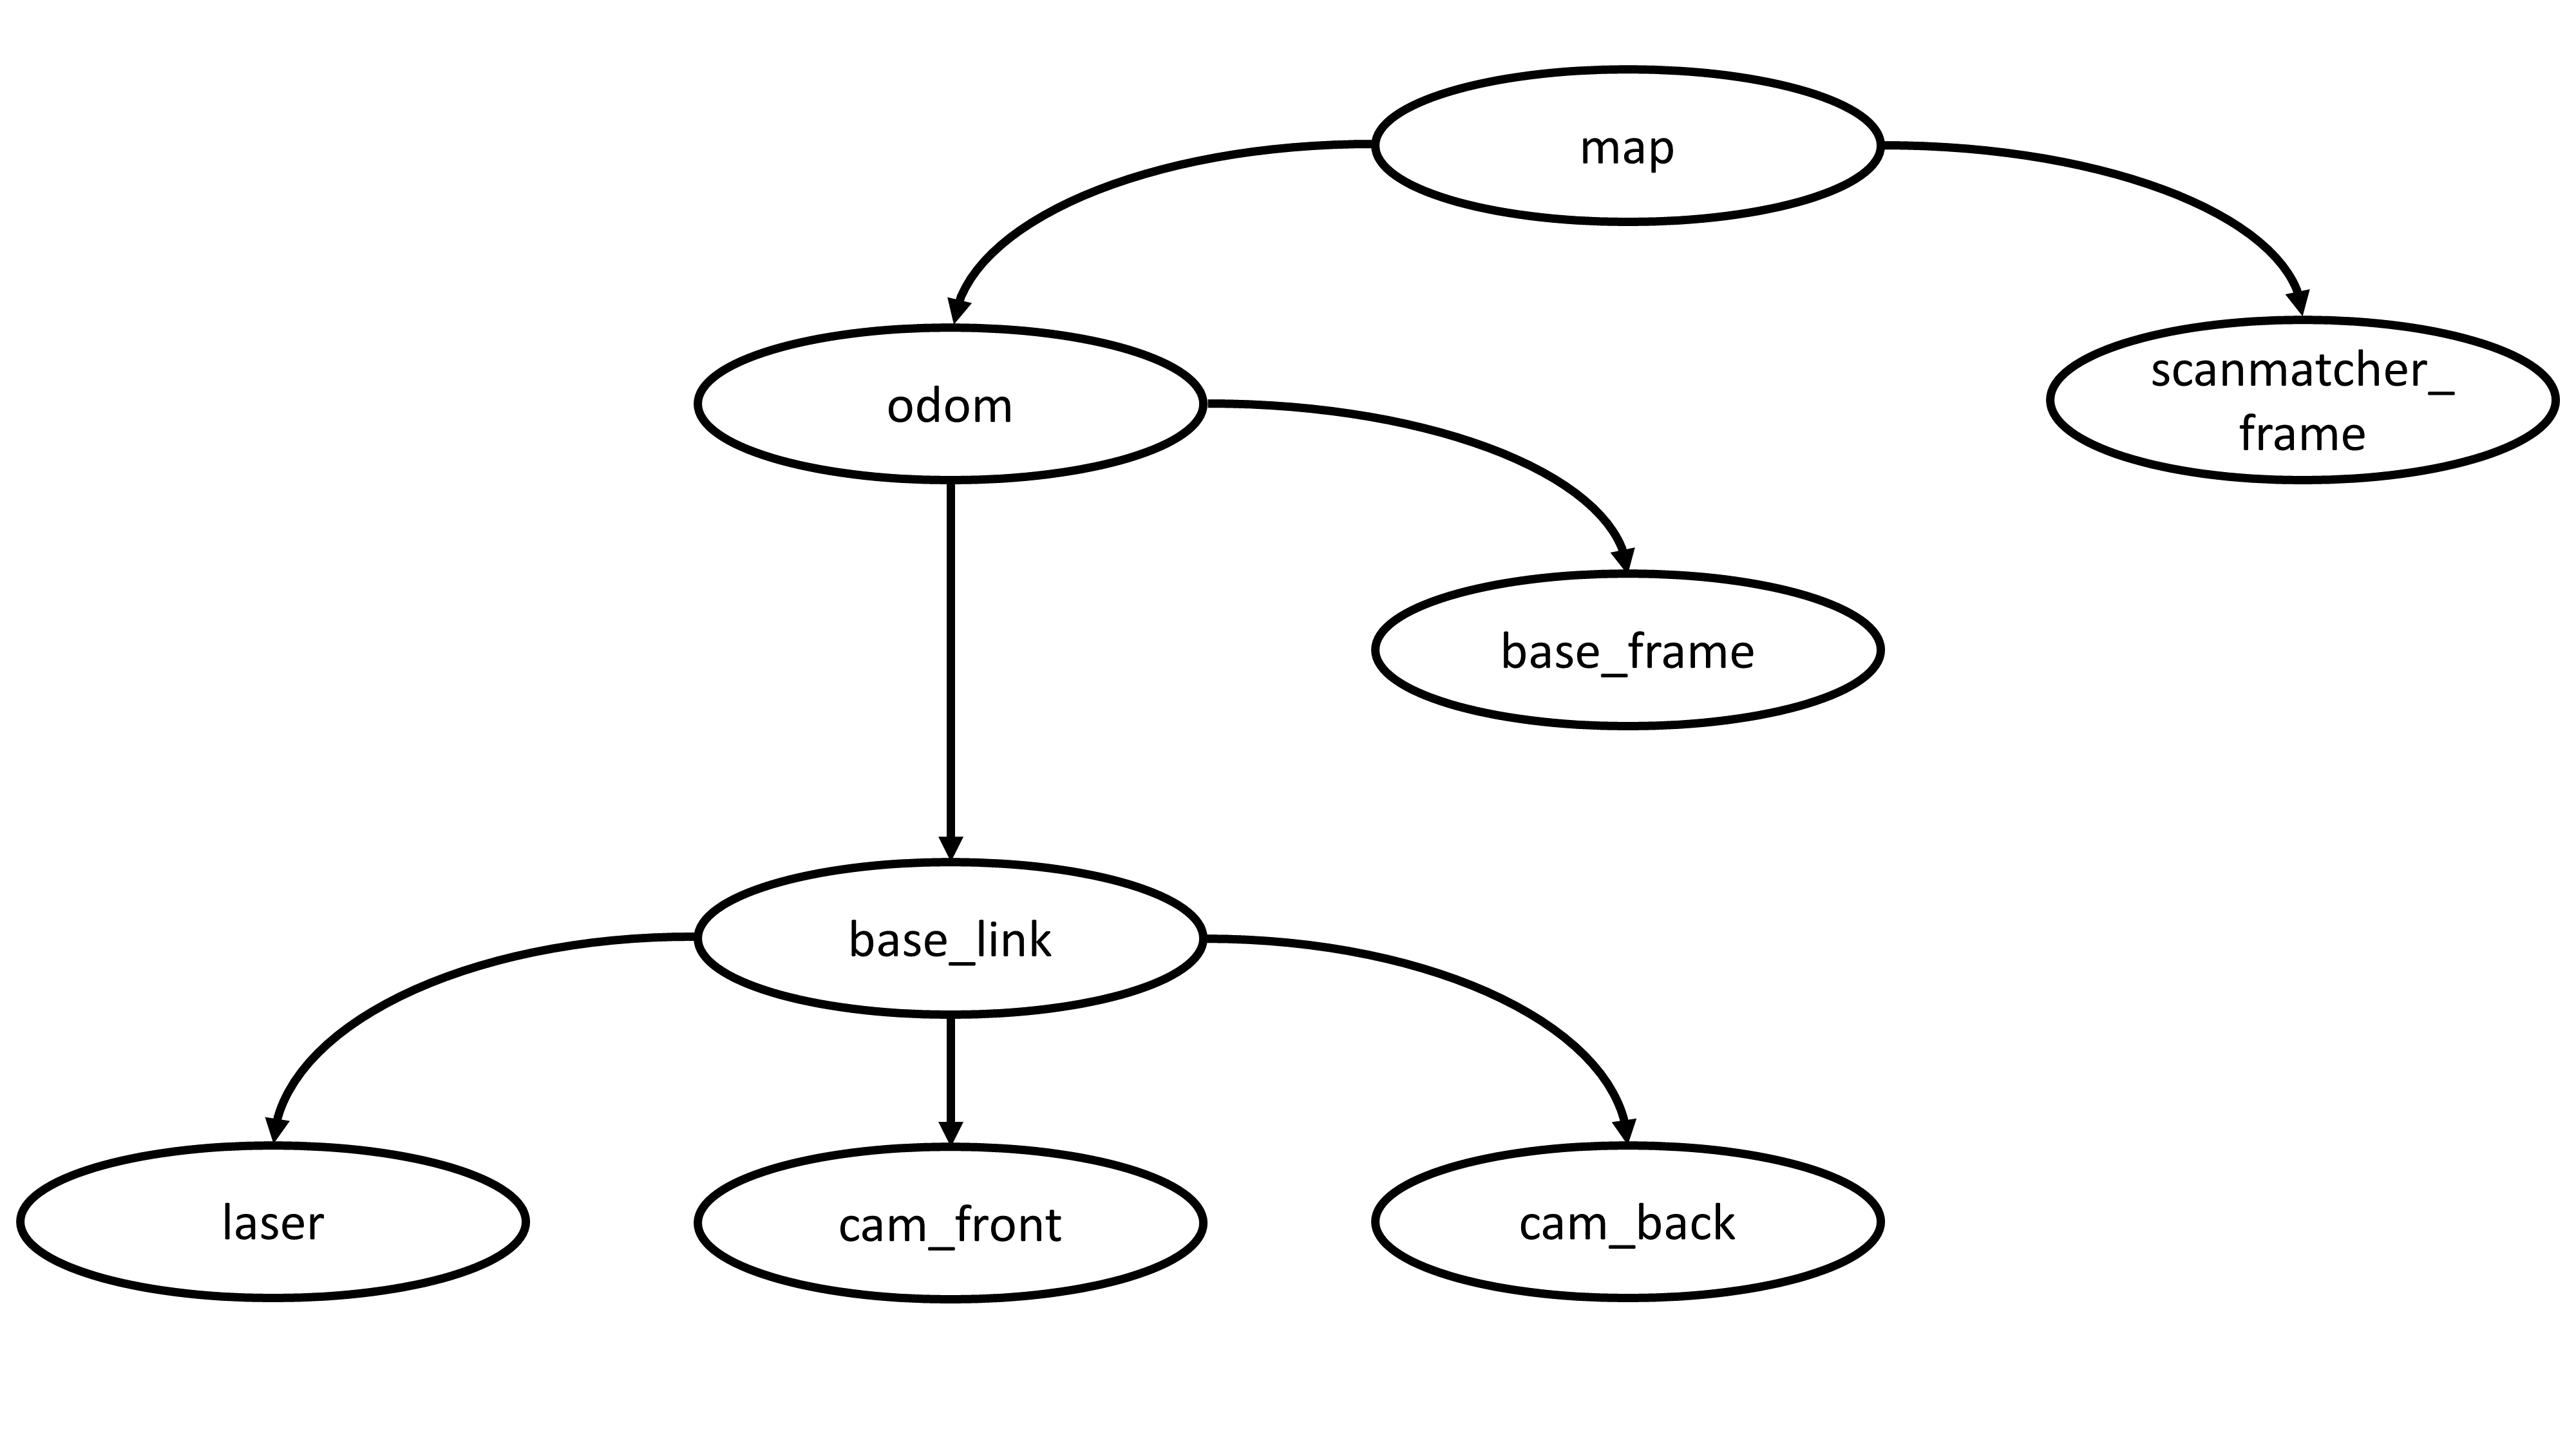
\includegraphics[width=1.0\textwidth]{Bilder/frames}
		   			\caption{Darstellung der Baumstruktur der in diesem Projekt verwendeten Koordinatentransformationen. Die Pfeile geben die Transformationsrichtung an. Die Umwandlungen von map$\rightarrow$odom und map$\rightarrow$scanmatcher\_frame sind dynamisch. Die Übrigen sind statische Transformationen.  }
		   			\label{fig: Baum der Koordinatentransformationen}
		   		\end{figure}
		      		    
		        Die in Abbildung \ref{fig: Baum der Koordinatentransformationen} dargestellten, dynamischen Transformationen map $\rightarrow$ odom und map $\rightarrow$ scanmatcher\_frame werden von \textit{Hector Slam} durchgeführt. Diese sind notwendig um die Verschiebung der Umgebung im Verhältnis zu dem Roboter darzustellen. Das Koordinatensystem \textit{odom} liegt an derselben Position wie \textit{base\_link}, \textit{laser} und der Sensor \textit{RPLIDAR A2}. \textit{Hector Slam} benötigt die Transformationen zwischen diesen Koordinatensystemen für die Kartografierung. Durch die Dokumentation dieses Knotens ist lediglich ein Bezug zwischen der Quelle der Sensorsignale und \textit{base\_frame} herzustellen \cite{hectorslam}. \textit{Rviz} meldet jedoch Fehler und weist den Benutzer auf die fehlenden Transformationen hin. Die \textit{Kinect}-Sensoren werden jeweils durch die Koordinatensysteme \textit{cam\_front} und \textit{cam\_back} beschrieben. Das \textit{base\_frame} beschreibt das Zentrum des Fahrzeugs und ist für eine Planung einer kollisionsfreien Trajektorie notwendig. Der \textit{Static Transform Publisher} veröffentlicht statische Koordinatentransformationen in das Topic \textit{tf}. \cite{sttrpu}
		 			    
		 			    
		    \section{Erstellung einer Trajektorie und der daraus folgenden Bewegungsbefehle}
		    \label{subsubsec: Erstellen der Bewegungsplanung}
		    	
		    	Mit den vorhandenen Sensordaten und dem Abbild der Umgebung aus den Kapiteln \ref{subsec: Auswerten der Sensordaten} und \ref{subsec: Kartografierung und Bewegungsplanung} können Trajektorien geplant werden. Die aus dieser Planung entstehenden Bewegungsbefehle werden durch die in Kapitel \ref{sec:Schlupfregelung} beschriebene Regelung in Bewegungen des Fahrzeugs umgesetzt.
		    
		    	\subsection{Bestimmung der Bewegungsbefehle}
		    	\label{subsec: Bewegungsbefehle}
		    	
		    	Das Softwarepaket \textit{Navigation} enthält Funktionen für die Umwandlung einer Zielpose in Geschwindigkeitsbefehle. Die Hauptanwendung des Pakets ist der Knoten \textit{Move Base}. Dieser abonniert Observationsquellen, eine \textit{Occupancy Grid}-Karte, Koordinatentransformationen oder Odometrieinformationen und 2D-Zielposen aus dem ROS-Netzwerk. Der Knoten veröffentlicht ein Bewegungsbefehl und \textit{Costmaps}, die in Abschnitt \ref{subsec: Einfluss der Umgebung auf die Planung einer Trajektorie} erläutert werden. \cite{navigation,movebase}\\ 
		    	
		    	In dieser Bachelorarbeit abonniert \textit{Move Base} die Topics \textit{Scan}, \textit{Scan1} und \textit{Scan2} von den in Kapitel \ref{subsubsec: Übersetzen der Laserdaten} und \ref{subsubsec: Kinect-Sensor} beschriebenen Observierungsquellen. Des Weiteren werden die Informationen über Koordinatentransformationen und 2D-Zielposen aus den Topics \textit{tf} sowie \textit{/move\_base\_simple/goal} abonniert. In der Abbildung \ref{fig: Rosnetwork} sind alle Abonnements und Veröffentlichungen des Knotens dargestellt.\\
		    	
		    	Der Knoten \textit{Move Base} ist in einzelnen Teilanwendungen aufgeteilt. Der enthaltene \textit{Global Planner} wandelt eine Zielpose in eine Trajektorie um. Durch einen externen Knoten, wie zum Beispiel \textit{Rviz}, kann ein solches Ziel im ROS-Netzwerk veröffentlicht werden. Aus der Trajektorie des \textit{Global Planners} und der geschätzten Position des Roboters erstellt der \textit{Local Planner} das Topic \textit{cmd\_vel}. Dieses beinhaltet eine Bewegungsplanung, resultierend aus der aktuellen Positionsschätzung und der geplanten Trajektorie und dient als Grundlage für die Erstellung des Bewegungsziels aus Kapitel \ref{subsec: Winkelregelung}. \cite{movebase,cmdvel}\\
		    	
		    	Der in diesem Projekt verwendete \textit{Teb Local Planner} gilt als Plugin für den in \textit{Move Base} vorhandenen \textit{Local Planner} und arbeitet nach der \textit{Timed Elastic Band} Methode (TEB). Durch eine prädiktive Regelung, die durch die TEB-Methode beschrieben ist, lassen sich Vorhersagen über die abzufahrende Trajektorie tätigen, die kontinuierlich optimiert wird \cite{tebmethode}. 
		    	Der \textit{Teb Local Planner} plant die Trajektorie in Abhängigkeit von dem Roboterumriss aus Abbildung \ref{fig: footprint} und der zugrunde liegenden \textit{Costmap}, die im folgenden erkärt wird. \cite{teblp}
		    	
		   
		   \subsection{Einfluss der Umgebung auf die Planung einer Trajektorie}
		   \label{subsec: Einfluss der Umgebung auf die Planung einer Trajektorie}	
		    \begin{figure}[H]
		    	\centering
		    	\includegraphics[width=0.8\textwidth]{Bilder/footprint.png}
		    	\caption{Darstellung des Fahrzeugs ALF aus der Draufsicht. Als rotes Rechteck ist der Roboterumriss gekennzeichnet. Der \textit{Inscribed Radius} ist mit $R_i$ und der \textit{Circumscribed Radius} mit $R_c$ beschrieben. Die Kreise entsprechen jeweils den Radien $R_i$ und $R_c$. Der Kreismittelpunkt ist der Ursprung des \textit{base\_frame} Koordinatensystems, das in Kapitel \ref{subsec: Kartografierung und Bewegungsplanung} durch den \textit{Static Transform Publisher} eingeführt wurde}
		    	\label{fig: footprint}
		  	  \end{figure}
		    
		     Der Roboterumriss ist als Parameter in den entsprechenden Knoten hinterlegt und wird beim Aufruf von Rviz sichtbar. Abbildung \ref{fig: footprint} stellt den Roboterumriss des ALFs dar und beinhaltet die Radien $R_{i}$ und $R_{c}$ , die als \textit{Inscribed}- und \textit{Circumscribed} Radius bezeichnet werden und für die Erstellung der Costmap von Bedeutung sind \cite{costmap}. Das Softwarepaket abonniert, wie in Kapitel \ref{subsec: Auswerten der Sensordaten} erörtert, die Sensordaten aus der Umgebung und verarbeitet diese zu einer sogenannten Costmap. Diese Karte dient dazu die Zellen der in Kapitel \ref{subsec: Graph-basierende Techniken} beschriebenen \textit{Occupancy Grid}-Karte mit Werten, sogenannten Costs, zwischen 0 und 255 zu gewichten.
		  	Die \textit{Costmap} besteht aus mehreren Schichten, die unter anderem Daten über Gegenstände in der Hindernisschicht, Sicherheitsradien in der Inflationsschicht und bereits vorhandenen Karten in der statischen Schicht enthält. In der statischen Schicht wird die oben genannte \textit{Occupancy Grid}-Karte hinterlegt, diese fungiert als Basis für die Costmap und deren Werteverteilung. In dieser Bachelorarbeit abonniert die statische Schicht das Topic \textit{Map} des in Kapitel \ref{subsec: Kartografierung und Bewegungsplanung} beschriebenen Knotens \textit{Hector Slam}.
		  	Die Hindernisschicht enthält die verarbeiteten Daten aus Kapitel \ref{subsec: Auswerten der Sensordaten}. Dadurch werden bei Anwesenheit von Hindernissen die entsprechenden Zellen der \textit{Occupancy Grid}-Karte mit den Wert 254 belegt. \cite{costmap}\\
		  	
		  	Die Inflationsschicht veröffentlicht Informationen über die Gewichtung umliegender Zellen eines eingetragenen Hindernisses auf Basis des Roboterumrisses und den Radien $R_{i}$ und $R_{c}$. 
		  	Die Gewichtung sinkt mit steigendem Abstand zum \textit{Inscribed Radius} in Form einer $e$-Funktion und wird mit Gleichung (\ref{eq: cost}) berechnet. Der Funktionsverlauf kann von einem Anwender in einer Launchfile durch den Roboterumriss, die ROS-Parameter \textit{Cost Scaling Factor} und  \textit{Inflation Radius} beeinflusst werden.
		  	In der Gleichung (\ref{eq: cost}) ist die Distanz zur besetzten Zelle mit $r$ der \textit{Cost Scaling Factor} der $e$-Funktion mit $f$ und der \textit{Inscribed Radius} als $R_{i}$ definiert. \cite{costmap,inflation}
		  		
		  		\begin{equation}
		  		cost(r)=\left\{\begin{array}{ll} 253, & r\le R_{i}  \\
		  		e^{-f (r - R_{i})} \cdot 253, & r> R_{i}\end{array}\right.
		  		\label{eq: cost}
		  		\end{equation}\\		  	
		  	Sämtliche Werte, von der belegten Zelle bis zum \textit{Inscribed Radius} haben den Betrag 253. Erst ab der Distanz $r=R_{i}$ erfolgt die Werteverteilung nach der $e$-Funktion.
		  		
		  		Die drei Radien haben folgende Bedeutung:\\
		  		
		  		\begin{itemize}
		  			\item \textit{Inscribed Radius}: Es gibt definitiv eine Kollision mit dem eingetragenen Gegenstand, wenn das Zentrum des Roboters auf einer Zelle mit dem Wert 253 steht. Das Zentrum des Roboters entspricht den Bezugskoordinatensystem des Roboterumrisses.\\
		  			
		  			  			
		  			\item \textit{Circumscribed Radius}: Ähnlich dem \textit{Inscribed Radius}, jedoch ist eine Kollision mit dem Gegenstand abhängig von der Orientierung des Roboters. \\
		  			
		  			\item \textit{Inflation Radius}: Die Entfernung zum Gegenstand, mit der die Werteverteilung aus Gleichung (\ref{eq: cost}) endet. Die Entfernung zum Gegenstand vom \textit{Circumscribed Radius} bis zum \textit{Inflation Radius} dient als Pufferzone. Steht das Roboter in dem Bereich zwischen\textit{ Circumscribed} und \textit{Inflation Radius}, so kollidiert der Roboter definitiv nicht mit dem in der \textit{Occupancy Grid}-Karte eingetragenen Gegenstand.\newline
		  		\end{itemize}
		  			    	
		    	
		    	Eine Funktionsauswertung und Auftragen der Werte über r mit dem Radius $R_{i}=0.36\text{ } \si{m}$ aus Abbildung \ref{fig: footprint} und einen Faktor $f=10$ ergibt den Funktionsverlauf aus Abbildung \ref{fig: costverteilung}.
		    	
		   
		   
		   		\begin{figure}[H]
		   	\centering
		   	\begin{tikzpicture}[
		   	]
		   	\begin{axis}[
		   	width=12cm,
		   	height=7cm,
		   	grid = both,
		   	grid style={line width=.1pt, draw=gray!10},
		   	axis y line*=left,
		   	ticklabel style={% gilt für x und y
		   		/pgf/number format/.cd,
		   		use comma,% Komma als Dezimaltrenner
		   		1000 sep = {}% keine Tausendertrennung 
		   	},
		   	xlabel={$\text{Distanz } \textit{r} \text{ in Meter}$},
		   	ylabel={Wertverteilungsfunktion $costs(r)$},
		   	axis x line*=bottom,
			   xmin=0,	xmax=1, 
		   	ymax=300,
		   	legend pos=north east,
		   	]
		   %	\addlegendimage{/pgfplots/refstyle=plot4};
		   	\addplot[black, line width=0.8pt]  table [col sep=comma] from {costs.csv};
		   	\addlegendentry{costs(r)}
		   	\end{axis}
		   	\end{tikzpicture}
		   \caption{Verteilung der Werte über die Distanz r. Der \textit{Circumscribed Radius} liegt bei $\approx0.78\text{ }\si{m}$ und der \textit{Inflation Radius} bei $0.8\text{ }\si{m}$. Die Distanz von der besetzten Zelle $r=0\text{ }\si{m}$ bis zum \textit{Inscribed Radius} $r=0.36\text{ }\si{m}$ erhält den Wert 253, die restliche Werteverteilung entspricht dem Funktionsverlauf aus Gleichung (\ref{eq: cost}) mit den definierten Parametern.} 
		   \label{fig: costverteilung}
		   \end{figure}

		    
		    		
		    
		    
		    
		    Abbildung \ref{fig: trajektorie} zeigt eine vom \textit{Teb Local Planner} geplante Trajektorie in einer \textit{Costmap}. Die Zielpose wurde in \textit{Rviz} manuell in für das System unbekanntes Gebiet gelegt. Die Planung der Trajektorie berücksichtigt die im System bekannten Gegenstände, wie in Abbildung \ref{fig: trajektorie} zu erkennen ist. In der Abbildung ist die eingegebene Zielpose als grüner Pfeil in unbekanntem Gebiet, die vom \textit{Teb Local Planner} geplante Trajektorie als rote Pfeile. Der Roboterumriss des Fahrzeugs wird als grünes Rechteck dargestellt und stimmt mit dem Robotermodell überein.
		    
		    \begin{figure}[H]
		    	\centering
		    	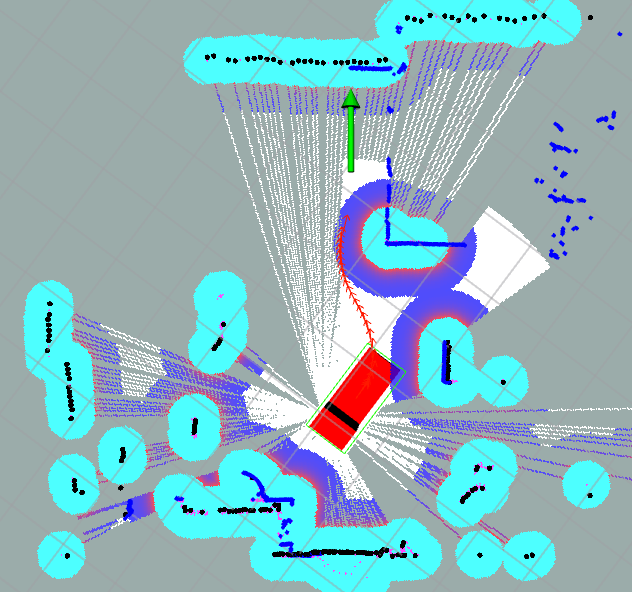
\includegraphics[width=0.8\textwidth]{Bilder/trajektorie.png}
		    	\caption{Darstellung einer \textit{Costmap} mit eingetragener Trajektorie aus der Draufsicht. Anhand der blauen und schwarzen Punkte erkennt man die visualisierten Sensorsignale, wie bereits in Abbildung \ref{fig: Verifikation der erfassten Laserdaten} veranschaulicht. In der Darstellung sind um diese Punkte die Gewichtungen der Costmap farblich markiert. Als Kette aus roten Pfeilen ist die abzufahrende Trajektorie dargestellt. Oben im Zentrum des Bildes repräsentiert ein grüner Pfeil die Roboterzielpose. Das grüne Viereck in der Mitte zeigt den Roboterumriss. Die vom Roboter ausgehenden Linien und Flächen demonstriert die Karte aus dem Topic \textit{map}.}
		    	\label{fig: trajektorie}
		    \end{figure}
	    
	    
	    	Neben der Eingabe einer Zielpose in \textit{Rviz} oder den manuellen Verfahren des Fahrzeugs mit dem Joystick, ermöglicht der Knoten \textit{Explore Lite} eine automatisierte Erkundung der Umgebung. Dabei legt der Knoten die Zielposen in unbekannte Gebiete \cite{explorelite}. Durch das in Kapitel \ref{sec: Unterscheidung der Lenkungsprinzipien} beschriebene Lenkungsprinzip ist eine Fahrt ohne Kollisionen gewährleistet. Der Knoten bewertet unbekanntes Gebiet der \textit{Costmap} als Grenze und versucht diese zu erkunden bis das erreichbare Umfeld vollständig untersucht ist \cite{explorelite}. 
		  

		
			
			
					    
		    